%----------------------------------------------------------------------------------------
%	PACKAGES AND OTHER DOCUMENT CONFIGURATIONS
%----------------------------------------------------------------------------------------

\documentclass[runningheads]{llncs}
\usepackage[titletoc,toc,page]{appendix}
\usepackage{lipsum}
\renewcommand{\appendixpagename}{\appendixname}
\renewcommand{\appendixtocname}{\appendixname}
\noappendicestocpagenum
\usepackage[spanish]{babel} % espanol, ingles
\usepackage[utf8]{inputenc} % acentos sin codigo
\usepackage[dvipsnames, table]{xcolor}
\definecolor{mygray}{gray}{0.9}
\usepackage{minted}
\usemintedstyle{friendly}
\usepackage{breakurl}
\usepackage{tabularx}
\usepackage{array, graphicx}
\usepackage{booktabs}
\usepackage{pifont}
\usepackage{changepage}
\usepackage{tabu}
\usepackage{bmpsize}
\usepackage{subcaption}
\usepackage{booktabs}% http://ctan.org/pkg/booktabs
\newcommand{\tabitem}{~~\llap{\textbullet}~~}
\usepackage{float}
\usepackage[hyphens]{url}
\usepackage{listings}
\usepackage{hyperref}
\usepackage{titlesec}
\usepackage{amssymb}
\setcounter{tocdepth}{4}
\setcounter{secnumdepth}{4}
\titleformat{\paragraph}
{\normalfont\normalsize\bfseries}{\theparagraph}{1em}{}
\titlespacing*{\paragraph}
{0pt}{3.25ex plus 1ex minus .2ex}{1.5ex plus .2ex}
\usepackage[export]{adjustbox}[2011/08/13]
\usepackage[square, numbers, comma, sort&compress]{natbib} % Use the natbib reference package - read up on this to edit the reference style; if you want text (e.g. Smith et al., 2012) for the in-text references (instead of numbers), remove 'numbers' 
\hypersetup{
    colorlinks=true,
    linkcolor=blue,
    filecolor=blue,      
    urlcolor=blue,
    citecolor=blue,
    pdftitle={Detector de Pivotes de Riego y Silobolsas en Imágenes Satelitales para aplicaciones agrícolas},
    pdfpagemode=FullScreen
} % Colors hyperlinks in blue - change to black if annoying


\begin{document}
\frontmatter % Use roman page numbering style (i, ii, iii, iv...) for the pre-content pages
\newcommand{\HRule}{\rule{\linewidth}{0.5mm}} % New command to make the lines in the title page
\selectlanguage{spanish}

%----------------------------------------------------------------------------------------
%	TITLE PAGE
%----------------------------------------------------------------------------------------

\begin{titlepage}
\begin{center}
\textsc{\LARGE Universidad Nacional de Córdoba}\\ % University name

\begin{figure}[htbp]
	\centering
		
\includegraphics[width=0.5\textwidth]{img/logo.png}
		\rule{35em}{0.5pt}
\end{figure}

\textsc{\Large Proyecto Integrador}\\[0.5cm] % Thesis type
\textsc{\Large Ingeniería en Computación}\\[0.5cm] % Thesis type

\HRule \\[0.4cm] % Horizontal line
{\LARGE \bfseries Detector de Pivotes de Riego y Silobolsas en Imágenes Satelitales para aplicaciones agrícolas
}\\[0.2cm] % Thesis title
\HRule \\[1cm] % Horizontal line

 
\begin{minipage}[t]{0.4\textwidth}
\begin{flushleft} \large
\emph{Autores: }{Gianfranco \textsc{Barbiani}, Loreley \textsc{Bustamante}}\\ % Author name - remove the \href bracket to remove the link
\end{flushleft}
\end{minipage}
\begin{minipage}[t]{0.4\textwidth}
\begin{flushright} \large
\emph{Director:}\\{Mg. Ing. Miguel \textsc{Solinas}} \\
 % Supervisor name - remove the \href bracket to remove the link  
\emph{Codirector:}\\{Dr. Ing. Miguel \textsc{Solinas} Jr.}
\\~\\~\\ % Supervisor name - remove the \href bracket to remove the link  
\end{flushright}
\end{minipage}

{\large \today}\\ % Date
\vfill
\end{center}
\end{titlepage}
\clearpage % Start a new page
\pagebreak

%--------------------------------------------------------
%	ABSTRACT
%--------------------------------------------------------
\begin{abstract}
En este Proyecto Integrador se diseñó e implementó una aplicación que hace uso de Machine Learning (ML) aplicado a la detección de objetos en imágenes satelitales para su aplicación en agricultura. Se describen las motivaciones, problemas encontrados y posibles soluciones. Se presentan principios de ML, deep learning y visión por computadora. Por último se presentan algunas conclusiones y futuros trabajos.
% En el presente proyecto integrador  se podrán identificar las etapas que componen el desarrollo de una aplicación que hace uso de Machine Learning. Se introducirán problemas, motivaciones y posibles soluciones para los mismos. Se expondrán principios sobre Machine Learning, Deep Learning y Visión por Computadora. A continuación habrá una sección sobre los riesgos relacionados al proyecto. Se detallarán las diferentes etapas del desarrollo e implementación de la aplicación así como también métricas, gráficos y figuras que demuestren el funcionamiento esperado de la misma. Al ultimo se concluye con una reflexión final sobre el proyecto, los problemas y limitaciones, y los futuros trabajos que se pueden originar.
\end{abstract}
\newpage

%--------------------------------------------------------
%	LIST OF CONTENTS/FIGURES/TABLES PAGES
%---------------------------------------------------------
\tableofcontents % indice de contenidos
\cleardoublepage

\listoffigures % Write out the List of Figures

\listoftables % Write out the List of Tables


%---------------------------------------------------------
%	THESIS CONTENT - CAPÍTULOS
%---------------------------------------------------------
\mainmatter % Begin numeric (1,2,3...) page numbering
\input{Chapters/Introducción}
\chapter{Marco Teórico}
\label{Marco Teorico}

\label{Principios de Machine Learning}
\section{Principios de Machine Learning}

Este trabajo integrador se incluyen campos de la inteligencia artificial, los cuales son Visión por Computadora y Deep Learning o Aprendizaje profundo. 
Esta sección tiene el propósito de hacer una introducción teórica a ambas ramas de la inteligencia artificial.

\subsection{Introducción: Visión por Computadora}
Una de las ramas de investigación más populares y utilizada de la Inteligencia Artificial es la Visión por Computadora o también llamada Computer Vision \cite{computervision1} \cite{computervision2} \cite{computervision3}.
Este campo se centra en intentar replicar funciones del sistema de visión humano, de forma que permita a las computadoras identificar y procesar objetos en imágenes o vídeos de forma similar a como los humanos lo hacen. Tiempo atrás, la capacidad de la visión por computadora era muy limitada, pero hoy en día hay muchas tecnologías que utilizan la visión por computadora, entre las cuales se encuentran el reconocimiento de objetos, la detección de sucesos, la reconstrucción de una escena y la restauración de imágenes.

En la actualidad, muchos son los campos que se han visto beneficiados por este conjunto de técnicas. Uno de los más conocidos es el de la robótica por medio de sensores o de cámaras, siendo estos últimos dispositivos idóneos para la aplicación de las estrategias de visión por computadora.

Sin embargo, podemos destacar otros ámbitos capaces de reconocer objetos, por ejemplo, en sistemas de seguridad, seguimiento de objetos o detección de anomalías en piezas fabricadas en una cadena de producción, medicina, etc.

\subsection{Fundamentos de Machine Learning}

Machine Learning \cite{ml}, es esencialmente un conjunto de algoritmos diseñado por un ser humano, pero que aprenden de los datos a los cuales son expuesto, dicho de otra manera, un conjunto de datos se usa para entrenar un modelo matemático de modo que cuando vea datos similares en el futuro, sepa reconocerlos. Los modelos, normalmente, toman datos como entrada y luego emiten una predicción de algo de interés. Estos algoritmos son ejecutados típicamente en algún tipo de computadora especial y sirven para resolver problemas de:
\begin{itemize}
    \item \textbf{Clasificación:} Retorna probabilidades de clase o distingue clases. Figura \ref{fig:clasificacion}.
    \item \textbf{Regresión:} Hace predicciones o estimaciones (en general numéricas). Figura \ref{fig:regresion}.
\end{itemize}

\begin{figure}[h!]
    \centering
    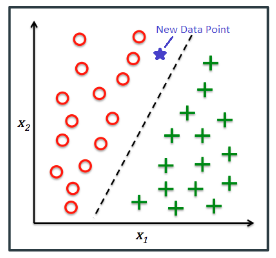
\includegraphics[width=0.5\textwidth]{img/clasificacion.png}
    \caption{Clasificación. Fuente: \cite{aprendisajesup}}
    \label{fig:clasificacion}
\end{figure}

\begin{figure}[h!]
    \centering
    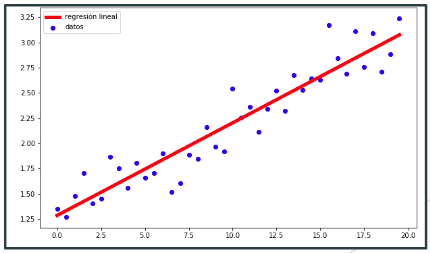
\includegraphics[width=0.8\textwidth]{img/regresion.png}
    \caption{Regresión. Fuente: \cite{aprendisajesup}}
    \label{fig:regresion}
\end{figure}

\newpage
El problema surge cuando se intenta resolver un problema de clasificación que no es linealmente separable. Aquí es donde aparecen la Redes Neuronales, con su capacidad de transformar estos problemas en linealmente separables. Figura \ref{fig:linealmente separables}.

\begin{figure}[h!]
    \centering
    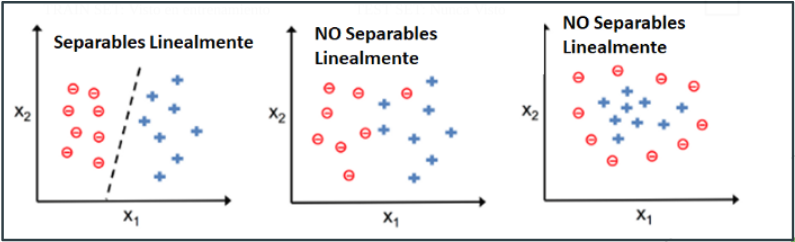
\includegraphics[width=1\textwidth]{img/linealmenteSeparable.png}
    \caption{Ejemplo Linealmente Separable. Fuente: \cite{aprendisajesup}}
    \label{fig:linealmente separables}
\end{figure}

\newpage
\paragraph{Ajuste del modelo: ¿Por qué se entrena un modelo de Machine Learning?}

Así como en la vida real a un ser humano se le enseña desde temprana edad a identificar distintos tipos de objetos dentro de su campo de visión, un modelo (o algoritmo) de Machine Learning tiene que aprender a detectar reconocer correctamente.

Para ello se lo entrena a partir de imágenes ya correctamente (ground truth) etiquetadas (bounding box) y, a grandes rasgos, si la predicción es correcta, se le alienta a seguir por ese camino y por el contrario si falla se lo alienta a ir en la dirección opuesta. Esto sería el ajuste con las perillas de una caja negra que viene a representar una abstracción de un modelo de Redes Neuronales, tal y como se representa en la siguiente Figura \ref{fig:abstraccion red neuronal}.

\begin{figure}[h]
    \centering
    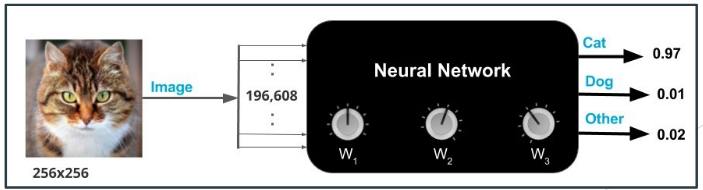
\includegraphics[width=1\textwidth]{img/RedNeuronal.png}
    \caption{Abstracción de una Red Neuronal. Fuente: \cite{redneuronalbasic}}
    \label{fig:abstraccion red neuronal}
\end{figure}

Se entrena el modelo a partir de un conjunto de datos lo suficientemente diverso, de tal manera que el modelo generalice y pueda realizar predicciones a partir de imágenes que nunca ``vio'' (analizó).

\begin{figure}[h!]
    \centering
    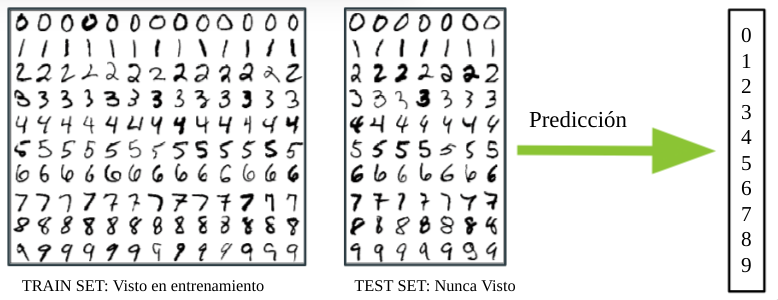
\includegraphics[width=1\textwidth]{img/RedNeuronal1.png}
    \caption{Ejemplo Machine Learning. Fuente: \cite{img_RedNeuronal1}}
    \label{fig:red neuronal 1}
\end{figure}

\subsection{Redes Neuronales}
Las Redes Neuronales Artificiales (ANNs por su siglas en inglés) son modelos matemáticos concebidos en un principio para estudiar (de cierta manera), el comportamiento del cerebro humano.
Estos modelos matemáticos son llamados Redes Neuronales porque fueron inspirados por neuronas biológicas, tal y como formalizaron: McCulloch y Pitts (1943) \cite{McCulloch1943-nf}; y Hebb & Hebb (1949) \cite{Morris1999-xd}. A grandes rasgos, se resume, que las Redes Neuronales Artificiales son formadas por circuitos neuronales y las interconexiones entre neuronas, llamadas sinapsis. Son llamadas sistemas conexionistas porque la información es codificada en los parámetros de las conexiones entre unidades.

En un principio, no hay una división clara entre conexionismo y neurociencia computacional, la principal diferencia es que los sistemas conexionistas se centran en procesos cognitivos de alto nivel, tales como: reconocimiento, memoria, comprensión  y razonamiento; en vez de detalles específicos del funcionamiento neuronal. En la década de 1980, el conexionismo experimentó una fuerte revitalización al formalizar una regla general de aprendizaje conocida como Backpropagation LeCun et al.(1988) \cite{lecun}. Backpropagation, que continua como el ``Hoyo en uno'' de la investigación conexionista contemporánea, permite a una amplia gama de modelos ANNs aprender una determinada función de mapeo de una entrada a una salida.

Hoy, el conexionismo esta mayormente englobado en el aprendizaje profundo (Deep Learning), ya que ha logrado  resultados notables en cuanto a avances en diversas aplicaciones. Aun no esta claro si las ANNs están limitadas en algún aspecto importante o no (por ejemplo, problemas de olvido catastrófico y ataques adversarios); sin embargo, está claro que los modelos de Deep Learning son lo suficientemente poderosos y flexibles para lidiar con muchos problemas.

En este capítulo, se introducen brevemente conceptos básicos relacionados al presente trabajo. Primero, se presentan las Redes Neuronales y su proceso de dos etapas (inferencia y entrenamiento). Luego, se introducen Clasificadores y otros modelos y técnicas esenciales para entender este trabajo. Finalmente, se presenta la literatura sobre Visión por Computadora y las métricas de evaluación centrales para medir la performance de los modelos de Machine Learning.

\subsection{Definición formal de Redes Neuronales}
En el aprendizaje supervisado, un dataset (conjunto de datos) de entrenamiento \mathbf{D = (xi, yi)}, representa a una función de mapeo (\mathbf{F : xi → yi}) definida por sus observaciones \textit{xi} y su correspondiente etiqueta \textit{yi}, que son variables independiente e idénticamente distribuidas (i.i.d) de una distribución \textit{Px},y. Luego, una red Neuronal es entrenada para aprender una función de mapeo \textit{f} que aproxima a \textit{F}. El objetivo de una Red Neuronal es relacionar correctamente las entradas \textit{xi} con las salidas \textit{yi}, mediante la adaptación de sus parámetros $\theta$. Por ejemplo, en un problema de clasificación de dígitos, \textit{xi} consiste en imágenes de dígitos mientras que \textit{yi} corresponde a la categoría del dígito.


En dos pasos, un clasificador de redes Neuronales aprende una función de mapeo \mathbf{y = f(x; $\theta$)} y adapta los parámetros $\theta$ que minimiza las predicciones del modelo y la verdad absoluta.

El primer paso se llama propagación Feedfoward o inferencia. La información de entrada \textit{x} fluye a través de la red Neuronal, siendo multiplicada por sus computaciones intermedias hacia la salida. En la mayoría de los casos, el mapeo \mathbf{f(x) : x → y},  es una función de activación descripta por \mathbf{f(x) : g3 ◦ g2 ◦ g1(x)} donde \textit{gl} son las capas intermedias conectadas en cadena \mathbf{y = f(x) = g3(g2(g1(x)))}. Las capas intermedias son parametrizadas por un vector de pesos \textit{$\theta$l}, que es utilizado para ponderar la entrada antes de ser transformadas por la función de activación. En cada capa oculta, la función de activación transforma la suma ponderada de las entradas en una salida. Las capas ocultas pueden también contener parámetros \textit{bias} que son utilizados usualmente para desplazar la suma ponderada de la entrada. Una capa es comúnmente representada como: \mathbf{gl(x) = φ($\theta$l, x)} donde \textit{$\theta$l} es el parámetro de la capa y \textit{φ} es la función de activación de la capa. Una red neuronal comprende de una capa de entrada \textit{g1}, que es la primer capa de la red, una capa de salida \textit{g3} y varias capas intermedias. La ultima capa, la capa de salida, es donde se espera que esté la predicción.
El largo total de esta cadena representa la profundidad del modelo y es de donde proviene el termino aprendizaje profundo (Deep Learning).

Los datos de entrenamiento provistos, comprenden de observaciones de F evaluados a diferentes puntos. Cada muestra \textit{xi} es acompañada de una etiqueta \textit{yi = F(xi)}, que representa la salida deseada para la capa de salida. En conjunto, la etiqueta especifica qué debe ser la capa de salida. Sin embargo, el comportamiento de salida de las capas intermedias no esta directamente especificado por los datos de entrenamiento, por eso se llaman capaz ocultas.

El segundo paso, es llamado entrenamiento y consiste en ``enviar hacia atrás'' (backpropagation), una señal de error sobre los parámetros del modelo (Riedmiller and Braun (1993) \cite{Riedmiller1993ADA}). Una función de pérdida (Loss function), es utilizada para computar el error cometido por el modelo en sus predicciones; esto es, la pérdida es alta cuando el modelo esta haciendo un trabajo pobre y por el contrario es baja cuando está performando bien. La señal de error, es el valor de la diferencia entre las etiquetas predichas y las verdaderas etiquetas deseadas. Luego, este valor de error, es utilizado para ajustar los parámetros del modelo para reducir la discrepancia en la predicción. El gradiente de la función de perdida con respecto a capas previas, es utilizado como la regla de actualización para ajustar los parámetros de cada capa. El proceso de aprendizaje es repetido hasta converger, por lo que un optimizador iterativamente computa el gradiente sobre lotes aleatoriamente muestreados del set de entrenamiento. Cuando una red neuronal encuentra un set de parámetros ``óptimo'', está lista para ser desplegada y comenzar así, a hacer predicciones sobre ejemplos nunca antes observados.

Un amplio rango de características (features), permiten a las ANNs, enseñarle a \textit{f} a encontrar un mapeo válido entre las entradas y las salidas. Por ejemplo, para evadir limitaciones lineales, funciones no lineales $\Psi$ son utilizadas en capas ocultas en vez de transformaciones lineales, ya que provee mayores grados de libertad, que habilitan al modelo a ``entender'' las relaciones no lineales entre los ejemplos \textit{x} y sus correspondientes etiquetas \textit{y}. Las transformaciones no lineales, permiten transformar problemas no linealmente separables en linealmente separables. Más específicamente, las funciones no lineales, permiten al espacio de entrada ser doblado, por lo que éste espacio puede ser dividido en regiones lineales más pequeñas (Pascanu et al.(2013) \cite{pmlr-v28-pascanu13}). La transformación no lineal, la correcta función de perdida y un apropiado número de parámetros en las capas ocultas, permiten a la red neuronal, aproximar cualquier función de mapeo. Éste es el origen del término aproximado universal (Hornik et al. (1989)). Para una introducción detallada de Redes Neuronales, por favor referirse a Hornik et al. (1989) \cite{HORNIK1989359}.

La función de mapeo aprendida \textit{f($\theta$, x)}, es actualizada y evaluada todo el tiempo en aprendizaje continuo. Cuando se evalúa la performance de un clasificador, lo que es juzgado detrás de escena, es el grado de degradación de la función de mapeo relativa a la función original de mapeo F.
    
\label{Principios de la Deteccion de Objetos}
\subsection{Principios de la Detección de Objetos}
Dentro de lo que es Computer Vision, existen diferentes aplicaciones para resolver una amplia gama de problemas:
\begin{itemize}
    \item \textbf{Object Clasification - Clasificación de Objetos:} Se determina si una imagen en su totalidad pertenece a una determinada clase.
    \item \textbf{Object Detection - Detección de objetos:} Se localizan y clasifican objetos de diferentes clases en una imagen. 
    \item \textbf{Image Segmentation - Segmentación:} consiste en dividir una imagen digital en varias regiones denominadas segmentos. Es un proceso de clasificación por píxel que asigna una categoría a cada píxel de la imagen analizada.
\end{itemize}

Con la ayuda de la siguiente imagen \ref{fig:computer vision} podemos entender mas fácilmente en qué consisten:

\begin{figure}[h!]
    \centering
    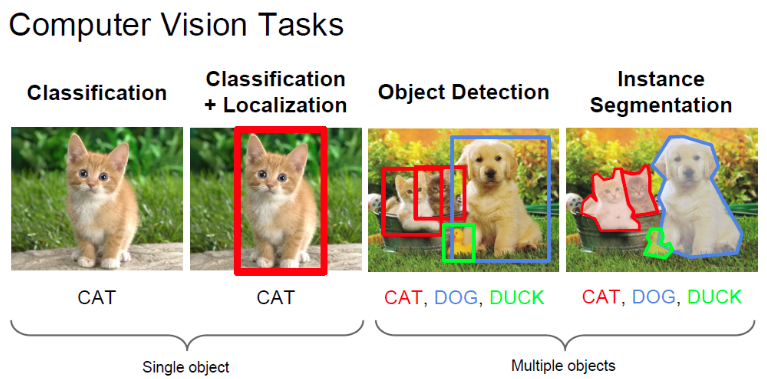
\includegraphics[width=0.8\textwidth]{img/computerVision.png}
    \caption{Tareas de Visión por computadora. Fuente: \cite{taskcompvision}}
    \label{fig:computer vision}
\end{figure}

\newpage
Este proyecto, optó por la \textit{Detección de objetos (Object Detection)} como herramienta principal para resolver la problemática de la identificación y localización de pivotes de riego y silobolsas en imágenes satélites, dada la naturaleza del problema: Hacer un conteo de la cantidad de estos objetos que se pueden encontrar en una determinada área de suelo.

\subsubsection{Conceptos}
Sin importar el modelo de Machine Learning subyacente, existen algunos conceptos dentro de lo que es Object Detection que son comunes a ésta aplicación y que ameritan ser explicados. Sin embargo, dado que el modelo seleccionado en este trabajo está basado en YOLO (You Only Look Once) \cite{yolo}, los conceptos a continuación se explican desde el punto de vista en el que son utilizados por YOLO.

\paragraph{Bounding box}
Cuando se realiza una predicción, el modelo ubica etiquetas (bounding box) en forma de recuadros sobre el objeto \cite{cnncourse}.

\begin{figure}[h!]
    \centering
    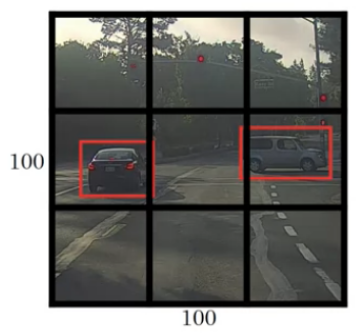
\includegraphics[width=0.6\textwidth]{img/bounding-box-yolo.png}
    \caption{Bounding Box in YOLO. Fuente:\cite{cnncourse}}
    \label{fig:bb in YOLO}
\end{figure}

YOLO divide la imagen en celdas, donde cada una de ellas se “encarga” de detectar los objetos cuyo centro de Bounding Box (BB) caiga dentro de ella. Figura \ref{fig:bb in YOLO} .

Cada celda arroja una salida con su predicción.
Dicha salida es un vector formado por: \[Y=\{Pc, Bx, By, Bh. Bw, C1, C2, C3\}\] con:
\begin{itemize}
    \item \textit{Pc = 0 o 1}: probabilidad de que haya un objeto en esa celda.
    \item \textit{Bx, By, Bh, Bw}: coordenadas (x, y, altura, ancho) para especificar el cuadro rojo delimitador del objeto asociado a esa celda.
    \item \textit{C1, C2, C3, …, Cn}: Probabilidades de las clases de objetos, por ejemplo puede ser las clases de peatón, coches y motocicletas.
\end{itemize}

\paragraph{Non-max suppression}
Es un algoritmo utilizado para que el modelo no detecte 2 veces el mismo objeto. Esto se debe a que YOLO realiza muchas predicciones sobre el mismo objeto, y de esta manera se realiza un filtrado seleccionando solo la mejor (Figura \ref{fig:non max supression}).
\\
\begin{figure}[h]
    \centering
    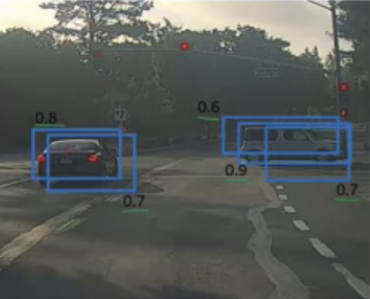
\includegraphics[width=0.6\textwidth]{img/non-max-supression-yolo.png}
    \caption{Non Max Supression in YOLO. Fuente:\cite{cnncourse}}
    \label{fig:non max supression}
\end{figure}

Procedimiento Non-max supression \cite{cnncourse} :
\begin{enumerate}
    \item Examina las probabilidades asociadas con cada una de las detecciones. 
    \item Selecciona el BB con el Pc más alto y lo elige como predicción parcial. Se descartan todos los BB con una \textit{Pc \leq 0.6}.

Si hay BB restantes:
    \item Descarta los BB remanentes con 0.5 o más de IoU contra el BB seleccionado en el punto anterior.
\end{enumerate}
Para el caso que haya varias clases, hay que correr Non-max una vez por cada clase, chequeando solamente los BB cuya predicción de clase sea la que se está chequeando en ese momento.

\newpage
\paragraph{Anchor Boxes}
Si dos o más objetos tienen el centro de su Bounding Box en la misma celda, el detector de objetos puede llegar a confundirse. Solución: Se pre-definen dos o más formas diferentes de cajas de anclaje o anchor boxes y se asocian tantas predicciones como anchor boxes haya. El anchor box que sea más similar a la forma del Bounding Box del objeto, será el asignado en el vector de salida \cite{cnncourse} (Figura \ref{fig:anchor boxes en YOLO}).

La elección de los tamaños y formas de los anchor boxes se puede elegir a mano, o tal vez 5 o 10 formas de anchor box, con una variedad suficiente como para cubrir todos los tipos de objetos que se quiere detectar.
También existe la posibilidad de realizar una selección más avanzada, es decir, automatizando la decisión, utilizando un algoritmo de machine learning llamado K-Means.
% \subsubsection{K-means}

\begin{figure}[p]
    \centering
    \begin{subfigure}[h!]{.4\textwidth}
        \centering
        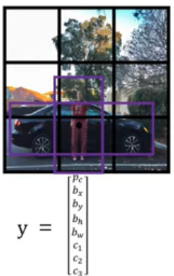
\includegraphics[width=\linewidth]{img/anchor-boxes-yolo-1.png}
        \caption{Output vector en YOLO}
    \end{subfigure}
    \begin{subfigure}[h!]{.6\textwidth}
        \raggedleft
        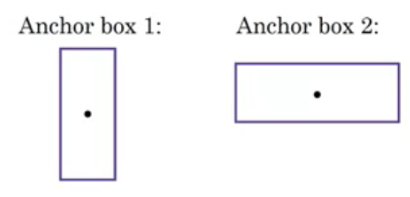
\includegraphics[width=\linewidth]{img/anchor-boxes-yolo-2.png}
        \caption{Ejemplos de Anchor Boxes en YOLO}
    \end{subfigure}
    \begin{subfigure}[h!]{.15\textwidth}
        \raggedright
        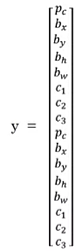
\includegraphics[width=\linewidth]{img/anchor-boxes-yolo-3.png}
        \caption{Output vector con 2 anchor boxes en YOLO}
    \end{subfigure}
    \caption{Anchor Boxes en YOLO.  Fuente:\cite{cnncourse}}
    \label{fig:anchor boxes en YOLO}
\end{figure}

\newpage
\paragraph{Intersection Over Union}
La intersección sobre la Unión o Intersection over Union (IoU) \cite{iou}, es una  métrica de evaluación utilizada para medir la precisión de un detector de objetos en un conjunto de datos en particular. Sin embargo, hay que tener  en cuenta que el algoritmo real utilizado para generar las predicciones no importa. Cualquier algoritmo que proporcione cuadros delimitadores predichos como salida, puede evaluar su rendimiento usando IoU; como por ejemplo, YOLO. Para aplicar IoU (Figura \ref{fig:iou 1}) y evaluar un detector de objetos (arbitrario), necesitamos:

\begin{itemize}
    \item Ground-truth bounding box (es decir, los cuadros delimitadores etiquetados ``a mano'' del conjunto de prueba que especifican en qué parte de la imagen está nuestro objeto).
    \item Predicted bounding box, cuadros delimitadores predichos de el modelo.
\end{itemize}

\begin{figure}[h!]
    \centering
    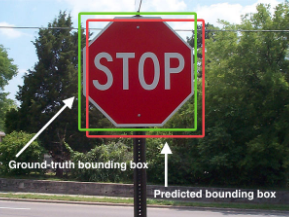
\includegraphics[width=0.6\textwidth]{img/iou-1.png}
    \caption{Ground Thruth and Predicted Bounding Box. Fuente:\cite{iou}}
    \label{fig:iou 1}
\end{figure}

El objetivo, es calcular la intersección sobre la unión entre estos cuadros delimitadores. Ésta intersección se puede determinar a través de la siguiente fórmula:  Figura \ref{fig:iou formula}:

\begin{figure}[h!]
    \centering
    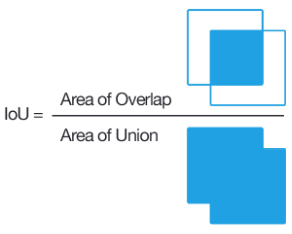
\includegraphics[width=0.5\textwidth]{img/iou-2.png}
    \caption{Intersetion over Union formula}
    \label{fig:iou formula}
\end{figure}

\newpage
\begin{itemize}
    \item En el numerador se calcula el  área de superposición entre el cuadro delimitador predicho y el cuadro delimitador de Ground-truth.
    \item El denominador es el  área de unión, o el área abarcada tanto por el cuadro delimitador predicho, como por el cuadro delimitador de Ground-truth.
\end{itemize}

Luego, dividir el área de superposición por el área de unión produce el puntaje final:  la Intersección Sobre la Unión - IoU. Una IoU mayor a 0.5 normalmente se considera una predicción ``buena''.

Cuando se entrena un detector de objetos, se necesita un conjunto de datos, que puede dividirse en dos grupos:

\begin{itemize}
    \item Un conjunto de entrenamiento utilizado para entrenar el detector de objetos.
    \item Un conjunto de pruebas para evaluar el detector de objetos.
\end{itemize}

Ambos conjuntos consistirán en:

\begin{itemize}
    \item Las imágenes en sí mismas.
    \item Los  cuadros delimitadores asociados con los objetos en la imagen, es decir, las coordenadas (x, y) del objeto en la imagen.
\end{itemize}

Estos cuadros delimitadores, para ambos conjuntos, están ``etiquetados a mano'' y, por lo tanto, son llamados ``ground-truth''. Su objetivo es tomar las imágenes de entrenamiento + cuadros delimitadores, construir un detector de objetos y luego evaluar su rendimiento en el conjunto de pruebas.

En la realidad, es  extremadamente  improbable que las  coordenadas (x, y) del Predicted bounding box coincidan exactamente con las coordenadas (x, y) del Ground-truth bounding box debido a los parámetros variables del modelo (como tamaño de ventana deslizante, método de extracción de características, etc.). Por ello, se necesita definir una métrica de evaluación que recompense los Predicted bounding box (rojo) por superponerse en gran medida con el Ground-truth (verde). 

\begin{figure}[h!]
    \centering
    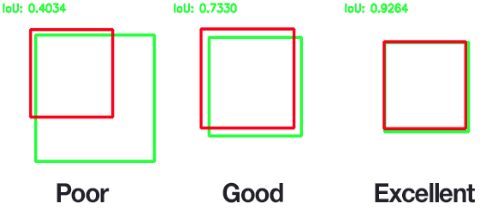
\includegraphics[width=0.6\textwidth]{img/iou-3.png}
    \caption{Intersetion over Union examples}
    \label{fig:iou ejemplos}
\end{figure}

Como se puede ver en la imagen \ref{fig:iou ejemplos}, los Predicted bounding box que se superponen en gran medida con los Ground-truth bounding box tienen puntajes más altos que aquellos con menos superposición. Esto hace que Intersection over Union sea una métrica excelente para evaluar detectores de objetos personalizados.


\newpage
\label{Dataset}
\subsection{Dataset}
En esta sección se detallan las especificaciones de los conjutnos de datos o datasets utilizados para entrenar el modelo YOLO.

\subsubsection{Pre-entrenamiento}
El modelo se entrenó desde cero (sus pesos establecidos aleatoriamente) usando el famoso dataset: VOC2012 Dataset \cite{voc2012}. Sus características principales son

\begin{itemize}
    \item Posee 20 clases. Figura \ref{fig:pascal-voc}
    \item Los datos de entrenamiento/validación contienen 11.530 imágenes comprendiendo 27.450 objetos anotados ROI (región de interés) y 6.929 objetos segmentados (no corresponde para object detection).
\end{itemize}

\begin{figure}[h!]
    \centering
    \begin{subfigure}[h]{\textwidth}
        \centering
        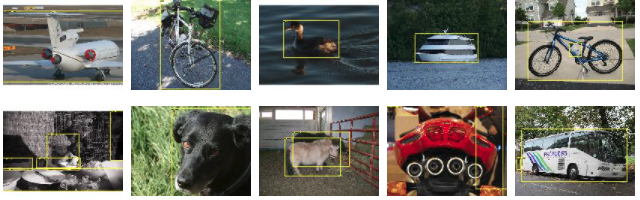
\includegraphics[width=\linewidth]{img/pascal-voc-20-classes-part1.png}
    \end{subfigure}
    \begin{subfigure}[h]{\textwidth}
        \centering
        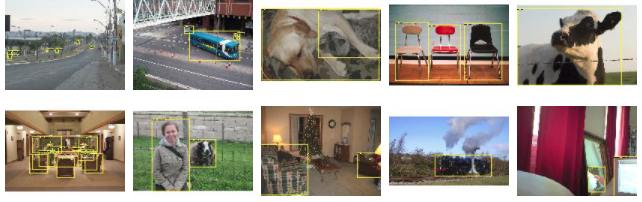
\includegraphics[width=\linewidth]{img/pascal-voc-20-classes-part2.png}
    \end{subfigure}
    \caption{Las 20 clases de VOC2012. Fuente: \cite{voc2012}}
    \label{fig:pascal-voc}
\end{figure}

\newpage
\subsubsection{Formato de las Etiquetas} 
Un dataset se compone típicamente de un conjunto de imágenes y un conjunto de etiquetas asociadas a cada una de ellas. Dichas etiquetas respetan un formato estricto, que para el caso del presente proyecto es: ``Pascal Visual Object Classes (VOC)'', el cual está caracterizado por:

\begin{itemize}
    \item Es un archivo XML. Ejemplo de formato VOC2012 \cite{etiqueta} :
    
        \lstset{frame=tb,
            language=XML,
            morekeywords={encoding,
                annotation,folder,filename,path,source,
                database,size,width,heigth,depth,
                segmented,object,name,pose,truncated,
                difficult,bndbox,xmin,ymin,xmax,ymax
            }
        }
        \begin{lstlisting}
        <annotation>
            <folder>Kangaroo</folder>
            <filename>00001.jpg</filename>
            <path>./Kangaroo/stock-12.jpg</path>
            <source>
                <database>Kangaroo</database>
            </source>
            <size>
                <width>450</width>
                <heigth>319</heigth>
                <depth>3</depth>
            </size>
            <segmented>0</segmented>
            <object>
                <name>kangaroo</name>
                <pose>Unspecified</pose>
                <truncated>0</truncated>
                <difficult>0</difficult>
                <bndbox>
                    <xmin>233</xmin>
                    <ymin>89</ymin>
                    <xmax>386</xmax>
                    <ymax>262</ymax>
                </bndbox>
            </object>
        </annotation>
        \end{lstlisting}
    \item Se crea un archivo para cada imagen del dataset.
    \item Las etiquetas están definidas como: \[(\textit{xmin-top left, ymin-top left, xmax-bottom right, ymax-bottom right})\]
\end{itemize}


% \begin{figure}[h!]
%     \centering
%     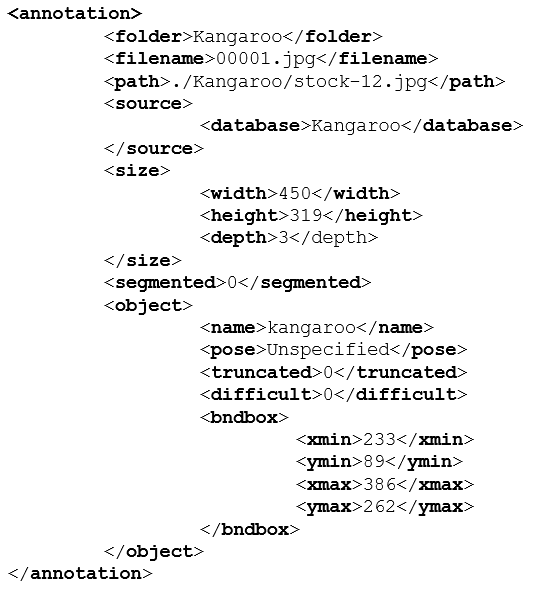
\includegraphics[width=0.7\textwidth]{img/pascal-voc-format-sample.png}
%     \caption{Ejemplo de formato VOC2012}
%     \label{fig:pascal-voc xml}
% \end{figure}

\newpage
\subsubsection{Dataset Personalizado}
El dataset con el cual se realizo el re-entrenamiento del modelo, esta basado en imágenes con vista satelital de pivotes y silobolsas extraídas de diferentes fuentes de acceso libre:
\begin{itemize}
    \item Usando la herramienta QGIS \cite{qgis} se obtuvieron imágenes satelitales de las fuentes: Sentinel, Google y Bing Sattelite.
    \item Google Maps
    \item Las etiquetas esta definidas como: \textit{(xmin-top left, ymin-top left,xmax-bottom right, ymax-bottom right)}
\end{itemize}

Las mismas poseen 3 bandas del espectro visible (RGB) y varían en tamaño, color, relación de aspecto de acuerdo a las diferentes estaciones del año y resolución, es decir, que tan cerca o lejos del nivel del mar se obtuvieron las imágenes. Se seleccionaron de tal manera que su distribución fuera uniforme: tantos objetos en solitario, como en conjunto, así como también balanceado, es decir, cada clase de objetos contenga la relativamente la misma cantidad.\\ 

La literatura y la práctica recomiendan un dataset “grande” para obtener resultados aceptables, lo que implica, como regla general:
\begin{itemize}
    \item Al menos 1500 imágenes por clase.
    \item Al menos 10000 instancias (objetos etiquetados) por clase.
\end{itemize}

Sin embargo ante la dificultad de seleccionar a mano un número tan grande de imágenes se optó por aplicar técnicas de Data Augmentation o Aumento de Datos, y de esta manera nos permite aumentar nuestro set de datos de entrenamiento para mejorar la precisión, la generalización, y controlar el overfitting:
\begin{itemize}
    \item Generación de Imágenes Sintéticas: Utilizando imágenes con diferentes colores y texturas como ``fondos'' e imágenes de los objetos de interés, se generaron nuevas imágenes sintéticas.
    \item Rotaciones: Se aplicaron rotaciones sobre las imágenes originales y las sintéticas
\end{itemize}

Finalmente el dataset quedó compuesto por decenas de miles de imágenes, algunas etiquetadas manualmente y en su gran mayoría imágenes similares a las que se muestran en el Anexo \ref{anexo:dataset}:

\newpage
\paragraph{Distribución de Etiquetas}
\begin{figure}[h!]
    \centering
    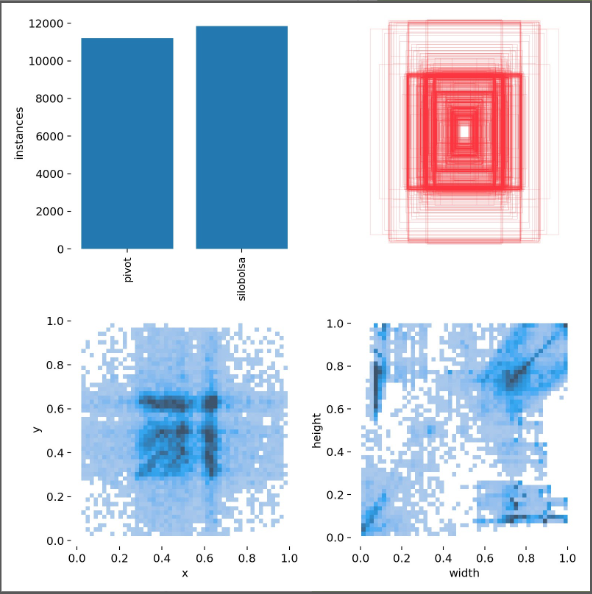
\includegraphics[width=0.95\textwidth]{img/distribucion de etiquetas.png}
    \caption{Distribución de Etiquetas}
    \label{fig:distribucion de etiquetas}
\end{figure}

De la anterior Figura \ref{fig:distribucion de etiquetas} se observan las siguientes conclusiones:
\begin{itemize}
    \item En el gráfico de barras ubicado en la esquina superior izquierda de la figura, se puede ver la distribución de etiquetas por clase. Notar que están relativamente balanceadas: con casi la misma cantidad de pivotes que de silobolsas.
    \item En la imagen superior derecha , se ven en rojo los diferentes bounding box (BB) que suelen ser en su mayoría cuadrados perfectos (pivotes y silobolsas en diagonal) de gran tamaño o bien muy pequeños, por lo que se concentran en la esquina superior derecha (1,1) e inferior izquierda (0,0).
    \item También se denota una gran concentración de BB altos y angostos  en la esquina superior izquierda (0,1) y anchos y bajos en la esquina inferior derecha (1,0), los cuales se corresponden a etiquetas de silobolsas de grandes dimensiones ubicadas vertical y horizontalmente respectivamente.
    \item En el gráfico ubicado en la esquina inferior izquierda se observa que el centro de los BB suele concentrarse en el centro de las imágenes y sobre todo evitan las esquinas.
\end{itemize}

\paragraph{Correlograma de Etiquetas}
\begin{figure}[h!]
    \centering
    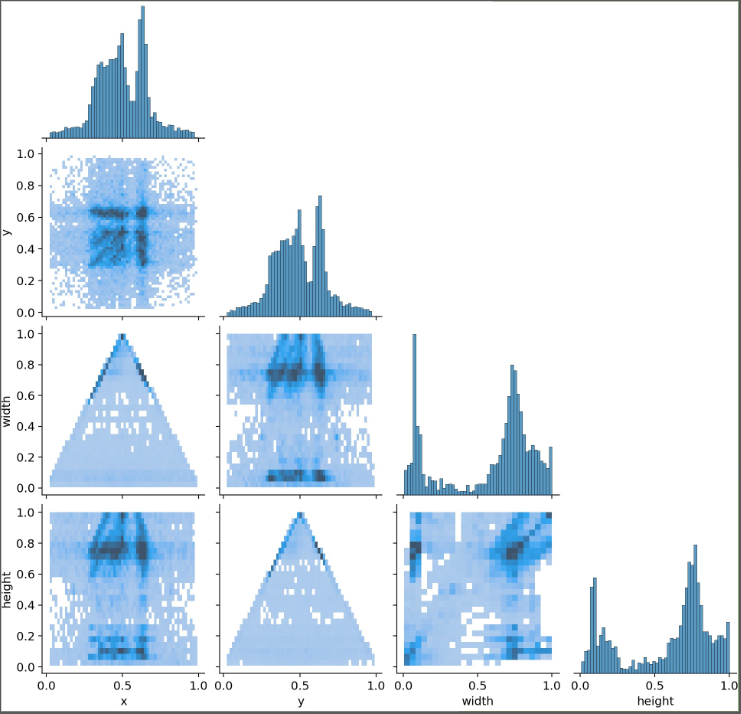
\includegraphics[width=1\textwidth]{img/correlograma de etiquetas.png}
    \caption{Correlograma de Etiquetas: nos ayudan a visualizar la correlación entre las etiquetas de los objetos. }
    \label{fig:correlograma de etiquetas}
\end{figure}

De la anterior Figura \ref{fig:correlograma de etiquetas} se observan las siguientes conclusiones:
\begin{itemize}
    \item La distribución de los BB se concentran en el centro de las imágenes, y sobre todo evitan las esquinas (x,y). 
    \item La distribución del ancho y alto de los BB denota que son cuadrados, o bien, rectángulos alargados tanto horizontales como verticales (width,height).
    \item Los BB ubicados en el centro del eje X de las imágenes tienden a ser extremadamente altas o bajas (x,height).
    \item Los BB ubicados en el centro del eje Y de las imágenes tienden a ser extremadamente anchas o angostas (y,width).
\end{itemize}


\newpage

\chapter{Estado del Arte}
\label{Estado del Arte - YOLO}

\section{Introducción}
En esta sección se tiene el propósito de hacer una distinción entre los principales tipos Detectores de Objetos. Hacer énfasis en el algoritmo de YOLO y sus variantes. Luego se exponen los Benchmarks (puntos de diferencia) entre los diferentes modelos más populares de detección de objetos y análisis del algoritmo de YOLO. La conclusión de la sección se lleva a cabo con la elección del modelo más conveniente para este proyecto.

\subsection{Detección de Objetos}

Dentro de las arquitecturas Deep Learning se distinguen dos ramas. La primera se conoce como arquitectura de dos fases, generando primero regiones candidatas de la localización del objeto en la imagen y posteriormente clasificando los objetos asignándole una categoría. Se los conoce por detectores de objetos basados en regiones, como los son: Fast R-CNN, Faster R-CNN y R-FCN. Mientras que este tipo de redes son el estado del arte en cuanto a precisión en la localización y clasificación de objetos, tienen la desventaja de ser demasiado lentas para la detección en tiempo real de objetos.

Por otro lado, el segundo tipo de detectores se conocen por tener una arquitectura de una sola fase. Estos realizan una abstracción mayor, donde ven el problema de detección de objetos como un problema de regresión (estimación de las cajas delimitadoras), como lo son SSD y YOLO. Debido a la necesidad de la capacidad de detección de objetos en tiempo real, surgieron las arquitecturas de un paso. Los expertos decidieron reducir el número de fases, logrando en una fase, arquitecturas capaces de inferir directamente a partir de una imagen las coordenadas de las cajas delimitadoras y la verosimilitud por clase. En esta sección, se presentará una de las arquitecturas de un paso usadas
para la detección de objetos en este proyecto.

\subsection{YOLO: You Only Look Once}
   Es uno de los algoritmos de detección de objetos en tiempo real más eficaces, que también abarca varias de las mejores ideas a través de toda la literatura de visión por computadora relacionada con la detección de objetos, por lo que resulta ser un Detector de objetos muy eficaz.
   YOLO \cite{yolo} plantea la detección de objetos como un único problema de regresión, directamente desde los píxeles de la imagen a las coordenadas de la caja delimitadora y a las probabilidades de cada clase, donde una sola red convolucional predice simultáneamente múltiples cajas delimitadoras y probabilidades de clase para esas cajas. YOLO se entrena en imágenes completas y optimiza directamente el rendimiento de la detección. Este modelo unificado tiene varios beneficios sobre los métodos tradicionales de detección de objetos:
   
   \begin{itemize}
        \item YOLO es extremadamente rápido.
            Al enfocar la detección como un problema de regresión, no se necesitan sistemas complejos. Simplemente se ejecuta la red neuronal en una nueva imagen para predecir las detecciones. Además, YOLO alcanza más del doble de la precisión media de otros sistemas en tiempo real.
        \item YOLO trabaja globalmente sobre la imagen. A diferencia de las técnicas de ventana deslizante y propuestas de regiones, YOLO ve toda la imagen durante el tiempo de entrenamiento y prueba, de manera que implícitamente codifica la información contextual sobre las clases, así como su apariencia.
        \item YOLO aprende representaciones generalizables de objetos. Cuando se entrena en imágenes naturales, YOLO es altamente generalizable, es menos probable que se descomponga cuando se aplica a entradas inesperadas por lo que supera los métodos de detección más avanzados
   \end{itemize}
   
   A pesar de estas ventajas, YOLO todavía se queda atrás en cuanto a la precisión con respecto a otros sistemas de detección. Aunque puede identificar rápidamente los objetos en las imágenes, tiene problemas para localizar con precisión algunos objetos, especialmente los pequeños. Esto resultó en un problema para este proyecto, debido a que los objetos de interés aparecen en la mayoría de las imágenes como objetos pequeños.
   
   YOLO \cite{yolo} (Lanzada:8 Junio 2015) ha ido publicando varias versiones, evolucionando desde la versión inicial, cuya estructura podemos ver en la Figura \ref{fig:yolo sistema}, hasta la última de ellas, YOLOv5 \cite{yolov5} - \cite{yolov5} lanzada el 18 Mayo 2020, la cual es una versión modificada de YOLOv4, pasando por las versiones YOLOv2 \cite{yolov2} (25 Diciembre 2016), YOLOv3 \cite{yolov3} (8 Abril 2018) y YOLOv4 \cite{yolov4} (23 Abril 2020).
   
   
\begin{figure}
    \centering
    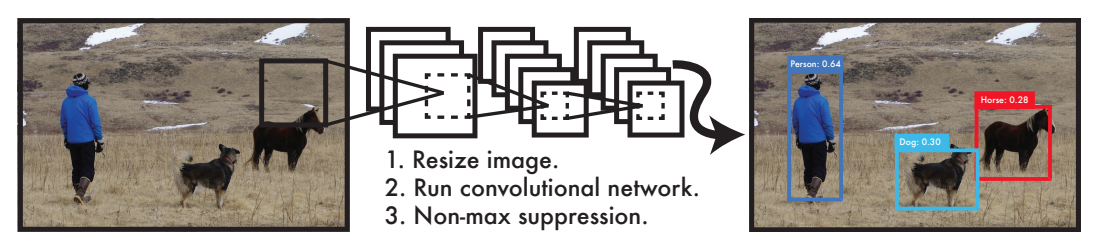
\includegraphics[width=0.9\textwidth]{img/Yolo1sistema.png}
    \caption{El sistema de detección de YOLO: Procesar imágenes con YOLO es simple y directo. El sistema (1) cambia el tamaño de la imagen de entrada a 448 × 448, (2) ejecuta una sola red convolucional en la imagen y (3) establece un umbral para las detecciones resultantes según la confianza del modelo. \cite{yolo}}
    \label{fig:yolo sistema}
\end{figure}
   
   
\subsubsection{Funcionamiento de YOLO}

La filosofía de las estructuras YOLO consiste en unificar los diferentes componentes de la detección de objetos en una sola red. El funcionamiento global de la inferencia, se puede ver en la siguiente Figura \ref{fig:yolo funcionamiento}.

\begin{figure}
    \centering
    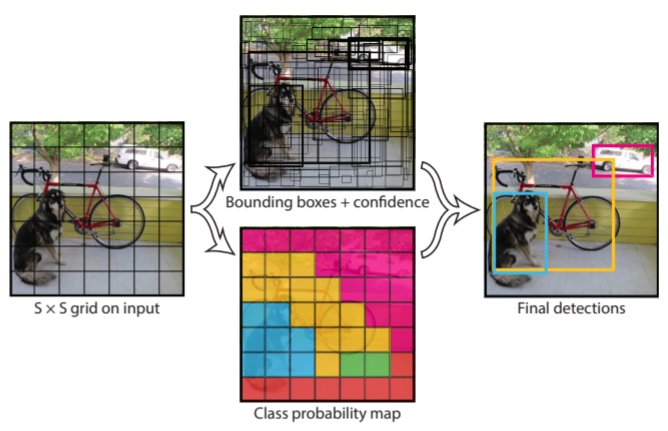
\includegraphics[width=0.9\textwidth]{img/YoloModel.png}
    \caption{Funcionamiento de YOLO: primero se divide la imagen en cuadrículas más pequeñas, sobre éstas se calculan diferentes cajas delimitadoras o bounding boxes y las probabilidades de las distintas clases que se encuentre en ellas, y finalmente se obtienen las detecciones. Fuente \cite{yolo}. }
    \label{fig:yolo funcionamiento}
\end{figure}

Los componentes principales para formar el algoritmo de detección de objetos YOLO:
    \begin{itemize}
         \item Intersection over Union
         \item Bounding Box Predictions
         \item Non-max suppression
         \item Anchor Boxes
    \end{itemize}

\paragraph{Workflow}
Para llevar a cabo la detección, utilizando YOLO:
\begin{enumerate}
    \item Primero, el algoritmo divide la imagen en una cuadrícula de tamaño SxS celdas (primera imagen de la izquierda Fig.\ref{fig:yolo funcionamiento}). Si el centro de un objeto cae en una celda de la cuadrícula, esa celda es la responsable de detectar el objeto.\\
    \item Cada una de las celdas detecta B posibles “bounding boxes” o cajas delimitadoras y calcula el nivel de certidumbre o confianza (probabilidad de la celda Pc) de cada una de las cajas (imagen del centro), que reflejan que tan seguro está el modelo de que esa caja contiene un objeto y qué tan seguro está de que efectivamente la caja se corresponde al objeto que ha detectado, es decir, se calculan SxSxB diferentes bounding boxes, la gran mayoría de ellas con un Pc muy bajo.
    \[Confianza = P(Objeto) ∗ IOU (truth prediction)\] Si no hay objeto en esa celda, la confianza debería de ser 0, en otro caso debería ser el IOU entre la caja detectada y la leída.\\
    \item Cada una de las cajas delimitadoras está compuesta por 5 predicciones: x, y, w, h y la confianza. Donde (x, y) representa las coordenadas del centro de la caja detectada y (w, h) el ancho y altura respectivamente.\\
    \item Además, cada celda de la cuadrícula también predice C probabilidades condicionales P(Clase \textit{i} $|$ Objeto), una por cada clase, que representan las probabilidades de que en esa celda se encuentre el objeto de la clase \textit{i}. Cabe remarcar, que se predice un vector de C probabilidades condicionales por cada celda, independientemente del número de cajas detectadas B.\\
    \item
    En la inferencia, se multiplican las probabilidades condicionales de cada clase y la confianza de cada caja detectada, obteniendo así las probabilidades específicas de cada clase por cada caja detectada e indicando la probabilidad de que cada clase aparezca en las cajas detectadas y qué tan bien se ajusta dicha caja.
\end{enumerate}


\subsubsection{YOLOv3}

A continuación se hablará de YOLOv3 \cite{yolov3}, que en un principio, fue el modelo elegido para el desarrollar este proyecto como una opción viable de llevarlo a cabo, y con el cual se realizaron las primeras pruebas y evaluaciones de los resultados. \\
Luego se mencionarán brevemente las mejoras que se implementaron en YOLOv3 con respecto a la primera versión YOLO, cuáles mejoras fueron implementadas en YOLOv2 y otras finalmente en YOLOv3.

\paragraph{Mejoras}
\begin{itemize}
    \item Normalización de los lotes en las capas convolucionales.
    \item Clasificador de alta resolución.
    \item Última capa convolucional con anchor boxes o cajas de anclaje, también llamadas cajas a priori. En vez de predecir directamente las cajas, se predicen los offsets con respecto a unas cajas de anclaje previamente predefinidas. Esto es muy útil por que se pueden definir dichas cajas de anclaje para que se adecuen mejor a la forma de los objetos del dataset.
    \item Clusters dimensionales: Como se ha mencionado, en muchos problemas de detección, los objetos tienen una forma determinada, por lo que para calcular las K cajas a priori que mejor cubren esta gama de formas en un dataset, se utiliza el algoritmo KMeans\cite{kmeans}.
    
    \textit{K-means} es un algoritmo de clasificación no supervisada (clusterización), que agrupa objetos en k grupos, basándose en sus características. El agrupamiento se realiza minimizando la suma de distancias entre cada objeto y el centroide de su grupo o cluster. Se suele usar la distancia cuadrática.
    \item Predicción directa de la localización
\end{itemize}

\textbf{Predicción de cajas delimitadoras} \\

Para la predicción de las cajas delimitadoras utiliza la misma metodología que YOLO9000 \cite{yolov2}. La red predice 4 coordenadas para cada anchor boxes \textit{(tx, ty, tw, th)}, de forma que si la celda de la cuadrícula tiene un offset con respecto a la esquina superior izquierda de la imagen de \textit{(cx, xy)} y la caja delimitadora a priori tiene anchura \textit{(pw, ph)}, entonces las predicciones finales son Figura \ref{fig:prediccion de bb}:


\begin{figure}[h!]
    \centering
    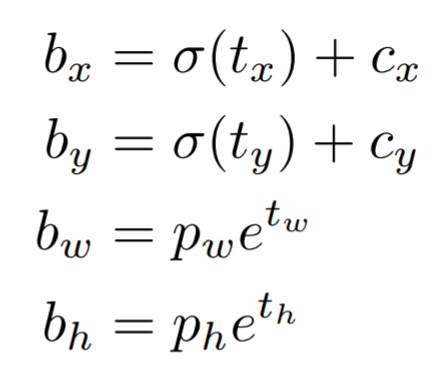
\includegraphics[width=0.25\textwidth]{img/BoundingBoxesFormula.png}
    \caption{Predicciones de las cajas delimitadoras}
    \label{fig:prediccion de bb}
\end{figure}

\newline
En otras palabras, la red predice offsets con respecto a cajas de anclaje (anchor boxes). Se puede ver en la siguiente Figura \ref{fig:cajas delimitdoras} una representación visual de estas ecuaciones. Esto es de mucha utilidad debido a que en muchos problemas de detección, los objetos tienen una forma determinada. Por lo tanto, se definen dichas cajas de anclaje para que se adecuen mejor a la forma de los objetos del dataset. Para calcular las K cajas a priori que mejor cubren esta gama de formas en un dataset, se utiliza el algoritmo K-Means sobre el dataset de entrenamiento.

\begin{figure}
    \centering
    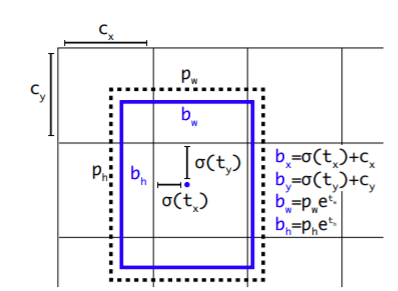
\includegraphics[width=0.7\textwidth]{img/BoundingBoxes.png}\\
    \caption{Cajas delimitadoras con dimensiones previas y predicciones. Se predice el ancho y la altura de la caja como offsets desde el centro de la caja.Fuente \cite{yolov3}}
    \label{fig:cajas delimitdoras}
\end{figure}
\\
Durante el entrenamiento se usa la suma de cuadrados como función de pérdida, de forma que el gradiente viene dado por \[\hat{t} \ast - t\ast \]  donde \[{\hat{t}\ast}\] es el offset predicho por la red y t∗ es el offset real.

\\ \break
YOLOv3 predice una puntuación de objeto para cada caja delimitadora usando regresión logística. Si el cuadro delimitador a priori no es la mejor, pero se superpone a un objeto por encima de un umbral (en este caso 0.5), se ignora la predicción. Es decir, después de obtener todas las predicciones, se procede a eliminar las cajas que estén por debajo de un límite, utilizando una medida que ayude a comparar la precisión de las predicciones del modelo (IoU $>$ 0.5).

A las cajas restantes se les aplica un paso de “non-max suppression”, que sirve para eliminar posibles objetos que fueron detectados por duplicado y así dejar únicamente el más exacto de ellos. \\


\textbf{Predicción de clases} \\

Cada casilla predice las clases que puede contener la caja delimitadora utilizando la clasificación multi-etiqueta, usando para ello, clasificadores logísticos independientes. Durante el entrenamiento se usa como función de pérdida la entropía cruzada binaria. \\


\textbf{Predicciones en diferentes escalas} \\

YOLOv3 realiza predicciones en 3 escalas diferentes. El sistema extrae características de cada una de estas 3 escalas, inspirado y utilizando un concepto similar a las redes piramidales de características o feature pyramid networks \cite{featurepiramid} (en VGG-16) Figura \ref{fig:vgg-16}. En la estructura, después de las capas de extracción de características en YOLOv3 se añaden diferentes capas convolucionales, la última de ellas es la encargada de predecir un vector 3D, codificando las predicciones de cajas delimitadoras, la probabilidad de contener un objeto y predicciones de clase. Así, el vector final es de la forma: \[N * N * (Nboxes ∗ (4 + 1 + Nclasses)\], donde \textit{Nboxes} es el número de cajas predichas en cada escala, \textit{4} se corresponde a los offsets (desplazamiento) de la caja delimitadora, \textit{1} a la predicción del objeto o probabilidad de contener un objeto y \textit{Nclasses} es el número de clases del dataset.

\begin{figure}
    \centering
    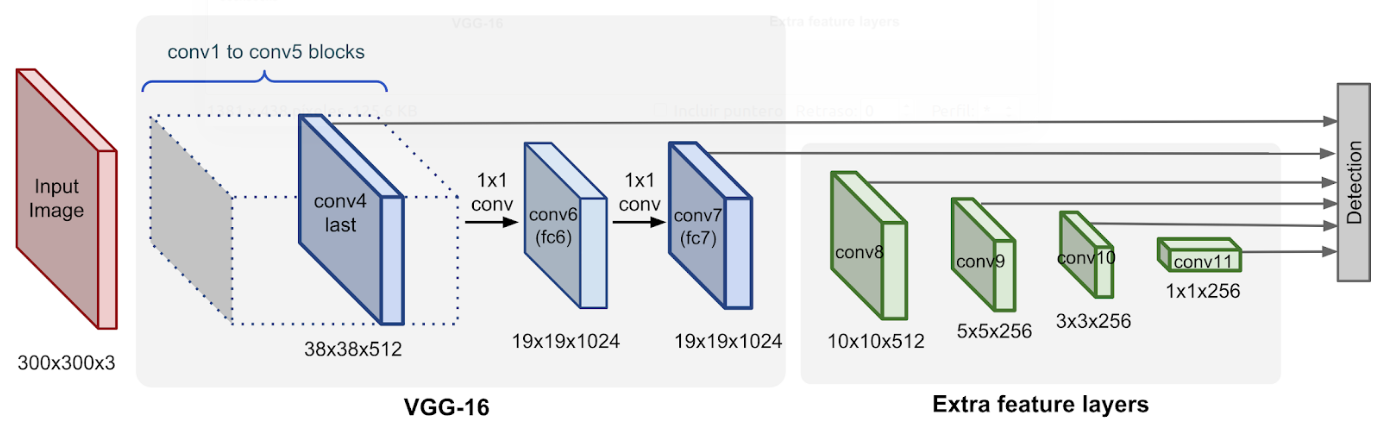
\includegraphics[width=1\textwidth]{img/VGG-16-NetPriamidal.png}
    \caption{Redes Piramidales de Características}
    \label{fig:vgg-16}
\end{figure}

Se toma el feature map o mapa de características de las dos capas anteriores y se aumenta en 2×. También se toma un mapa de características de las capas anteriores de la red y se fusiona con las características aumentadas de capas subsiguientes, usando concatenación. Este método permite obtener información semántica más significativa. Se realiza el mismo proceso una vez más para predecir cajas para la escala final. Así, las predicciones para la tercera escala se benefician de todos los cálculos previos. De esta manera, se ocupa de muchos más candidatos de bounding boxes de diferentes tamaños. \\


\textbf{Extractor de características} \\

Se utiliza un enfoque híbrido entre el extractor de características utilizado por YOLOv2 (Darknet-19) \cite{yolov2} y capas residuales. Utiliza capas convolucionales sucesivas de 3 × 3 y 1 × 1, con algunas interconexiones o atajos. Tiene 53 capas convolucionales en total y recibe el nombre de Darknet-53. Se puede ver un resumen de su estructura en la Figura \ref{fig:darknet-53}.

\begin{figure}[h!]
    \centering
    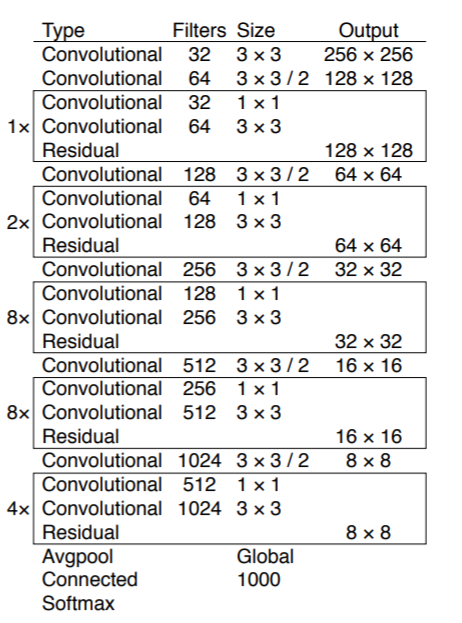
\includegraphics[width=0.6\textwidth]{img/Darknet53.png}
    \caption{Darknet-53}
    \label{fig:darknet-53}
\end{figure}

\newpage
\paragraph{Comparación con otras estructuras}
Se puede ver una comparación en los resultados finales con otras estructuras populares para la detección de objetos en la Figura \ref{fig:comparacion RN}.

\begin{figure} [h!]
    \centering
    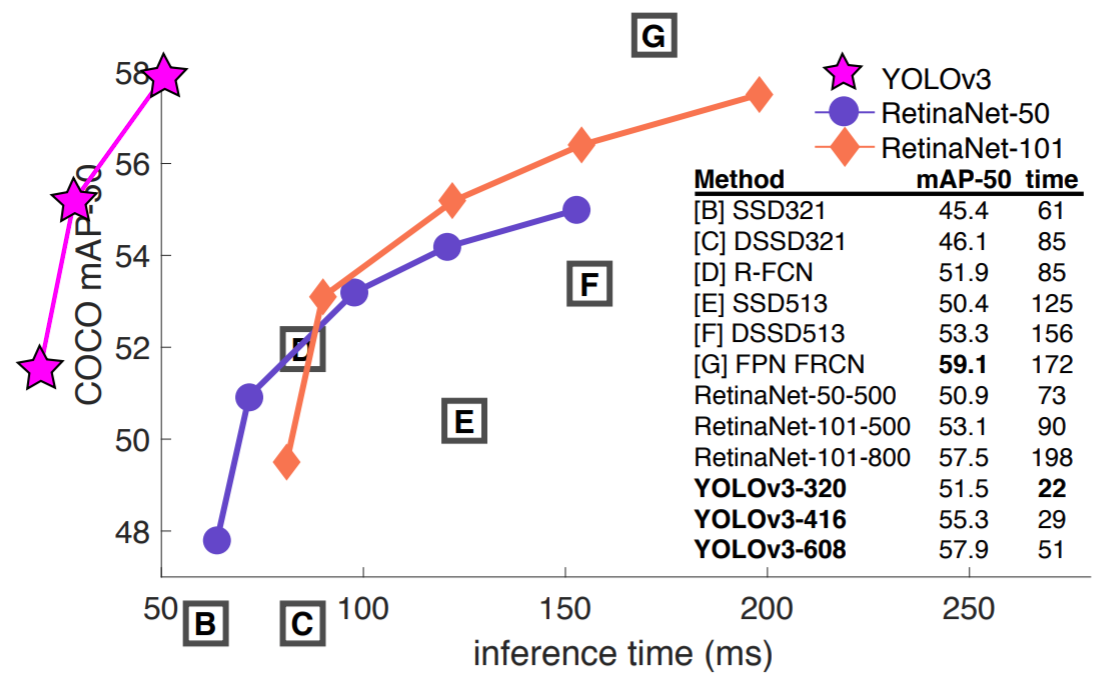
\includegraphics[width=1\textwidth]{img/ComparacionRN.png}
    \caption{Comparación de distintas estructuras de redes neuronales convolucionales: se observa el balance entre velocidad y precisión para 0.5 IOU, destacando YOLOv3 por su gran velocidad y manteniendo una buena precisión. Fuente\cite{yolov3}}
    \label{fig:comparacion RN}
\end{figure}

\newpage
\subsubsection{YOLOv4}

En esta sección se hablará de YOLOv4 \cite{yolov4}, que presenta mejoras considerables con respecto a su predecesor, YOLOv3, tanto en velocidad de inferencia como en precisión de en torno a un 10-12 por ciento, como se observa en la siguiente Figura \ref{fig:object-detection-arqui}.

Además se encuentra una descripción muy detallada junto a los parámetros que utiliza la red en este enlace \cite{yolov4info}. Sin embargo, aunque es una propuesta muy interesante para la detección de objetos en tiempo real por su gran velocidad en cuanto a FPS (Frames per second o Imágenes por segundo) y manteniendo una muy buena precisión con respecto a otros detectores de última generación, al momento de de la selección final del modelo a usar, se opto por la elección de YOLOv5, que es la ultima versión disponible de los YOLO, el cual tiene todas las ventajas de YOLOv4, que se mencionarán brevemente a continuación. 

\paragraph{Mejoras}

\textbf{Nueva Arquitectura} \\

La arquitectura de YOLOv4 se puede dividir en 3 partes:
\begin{enumerate}
    \item {Backbone: Basado en la CSPDarknet53}
    \item {Neck: Basado en SPP y PAN}
    \item {Head: YOLOv3}
\end{enumerate}

\begin{figure}
    \centering
    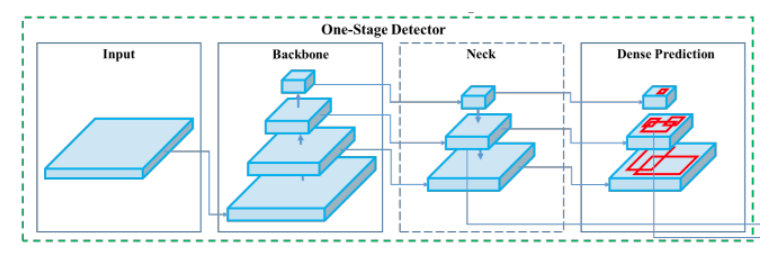
\includegraphics[width=1\textwidth]{img/ObjectDetectionArqui.png}
    \caption{Principales componentes de un Detector de Objetos moderno de una etapa.}
    \label{fig:object-detection-arqui}
\end{figure}

Esta nueva arquitectura trae nuevos beneficios con respecto a la versión anterior de YOLO, entre ellas se pueden mencionar que: 
\begin{itemize}
    \item Reduce en gran medida la cantidad de cálculo y mejorar la velocidad de inferencia y la precisión.
    \item Se ocupa de los siguientes tres problemas: Fortalecimiento de la capacidad de aprendizaje de una Red Neuronal Convolucional (CNN).
    Eliminación de cuellos de botella computacionales.
    Reducir los costos de memoria.
    \item Elimina el requerimiento de imagen de entrada de tamaño fijo.
    \item Otorga robustez frente a deformaciones de objetos.
    \item Aumenta el flujo de información propagada a través de la red.
    \item Mejora la predicción de la anchor boxes.
\end{itemize}
\hfill \break

\textbf{Bag of Freebies (BoF)} \\

Bolsa de regalos o Bag of Freebies se denomina al conjunto de técnicas o métodos que cambian la estrategia de entrenamiento o el costo de entrenamiento para mejorar la precisión del modelo. Permiten al detector de objetos ser más preciso sin incrementar el costo computacional, un ejemplo clásico es: data augmentation o el aumento de datos, es un técnica que permite crear variaciones artificiales sobre imágenes del dataset para expandir el conjunto de imágenes existentes y aumenta la capacidad de generalización del modelo.

Para ello se hacen distorsiones fotométricas como: cambiar el brillo, la saturación, el contraste y el ruido o hacer distorsiones geométricas de una imagen, como rotar, recortar, etc. Estas técnicas son un claro ejemplo de un BoF, y ayudan a mejorar la precisión del detector.

\begin{figure}[h!]
    \centering
    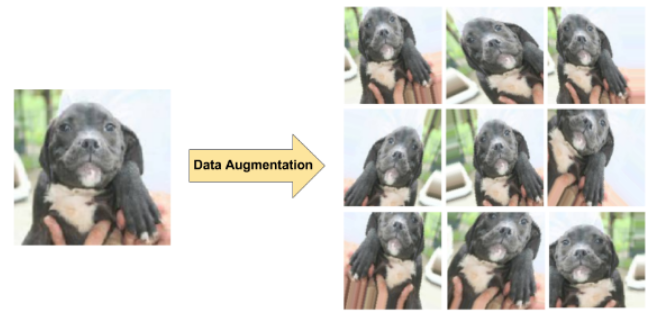
\includegraphics[width=1\textwidth]{img/dataAugmentation.png}
    \caption{Ejemplo de Aumento de datos \cite{dataaug}}
    \label{fig:data-augmentation-ejemplo}
\end{figure}

\begin{enumerate}
    \item {CutMix:}
    En lugar de simplemente eliminar píxeles como en Cutout Figura \ref{fig:cutmix}, se reemplazan las regiones eliminadas con un parche de otra imagen.
    Los parches agregados mejoran la capacidad de localización al requerir que el modelo identifique el objeto desde una vista parcial.
    No quedan píxeles no informativos durante el entrenamiento, lo que hace que el entrenamiento sea más eficiente.

    \begin{figure}[h!]
        \centering
        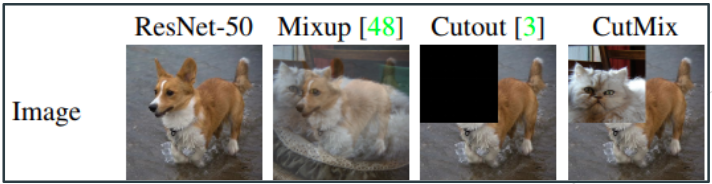
\includegraphics[width=0.9\textwidth]{img/cutMix.png}
        \caption{CutMix}
        \label{fig:cutmix}
    \end{figure}

    \item{Mosaic:}
    Combina 4 imágenes de entrenamiento en una sola, en ciertas proporciones (en lugar de solo dos en CutMix) (Figura \ref{fig:mosaic}).
    Permite que el modelo aprenda a identificar objetos a una escala menor de lo normal y mejorar así la precisión de sus modelos hasta en un 10\%. Combina clases que pueden no verse juntas en su conjunto de entrenamiento.
    
    \begin{figure}[h!]
        \centering
        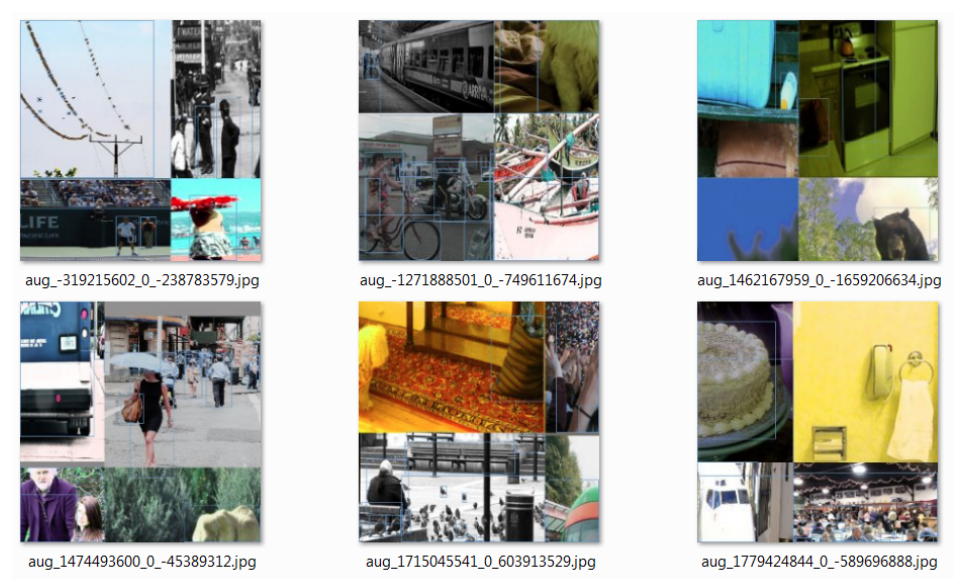
\includegraphics[width=0.8\textwidth]{img/mosaic.png}
        \caption{Mosaic representa un nuevo método de aumento de datos. \cite{yolov4}}
        \label{fig:mosaic}
    \end{figure}
    
    \item{Class label smoothing o Suavizado de etiquetas:}
    Es una técnica de regularización que aborda ambos problemas: overfitting (sobre ajuste) y exceso de confianza.
    Suavizar las etiquetas evita que la red se vuelva demasiado confiada.
    Ayuda al modelo a entrenarse en torno a datos mal etiquetados y, en consecuencia, mejorará su solidez y rendimiento.
    Matemáticamente, se altera el vector \textit{Y} de ground thruth por un factor $\alpha$:
    
    \begin{figure}[h!]
        \centering
        
\includegraphics[width=0.4\textwidth]{img/suavizadoEtiqueta.png}
        \label{fig:suavizado-etiqueta}
    \end{figure}
    
    \begin{figure}[h!]
        \centering
        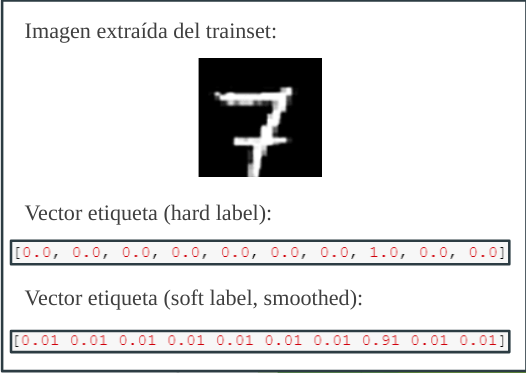
\includegraphics[width=0.8\textwidth]{img/suavizadoEtiquetaVector.png}
        \caption{Suavizado de Etiquetas}
        \label{fig:suavizado-etiqueta-vector}
    \end{figure}
\end{enumerate}
\hfill \break

\textbf{Bag of Specials (BoS)} \\

Como lo mencionan los autores \textit{Bag of Specials} contiene diferentes módulos y módulos de procesamiento posterior que solo aumentan el costo de inferencia en una pequeña cantidad, pero pueden mejorar drásticamente la precisión del detector de objetos. 

Hay muchos módulos diferentes presentes, pero en ésta parte solo se hace foco en uno de éstos métodos selectivos que se muestran en la Figura \ref{fig:bag-of-specials} y se responden el por qué de sus beneficios:

\begin{figure}[h!]
        \centering
        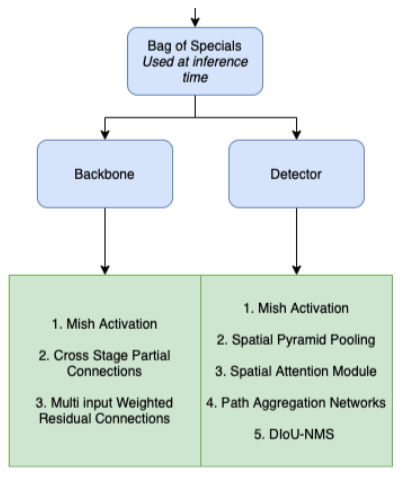
\includegraphics[width=0.8\textwidth]{img/BagOfSpecials.png}
        \caption{Diferentes métodos presentes en la Bag of Specials}
        \label{fig:bag-of-specials}
    \end{figure}

\begin{enumerate}
    \item {Módulo de Atención Espacial o Spatial Attention Model (SAM)}

    Se aplica una máscara de atención espacial a las features de entrada, para obtener un feature map refinado: Se destacan así las características más relevantes creadas por las capas convolucionales y se remueven las menos importantes. 
    Produciendo una mejora en la clasificación y la detección, con un costo computacional bajo.
    En YOLOv4, una versión modificada de SAM \cite{yolov4} es usada, en la cual no se aplica el maximum ni el average pooling. 
    \\
    
    \begin{figure}[h!]
        \centering
        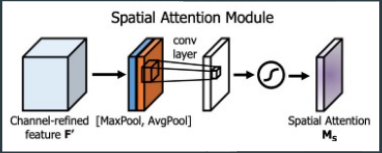
\includegraphics[width=0.8\textwidth]{img/SAM.png}
        \caption{Módulo de Atención Espacial \cite{sam1}}
        \label{fig:sam}
    \end{figure}
\end{enumerate}

    \begin{figure}[h!]
        \centering
        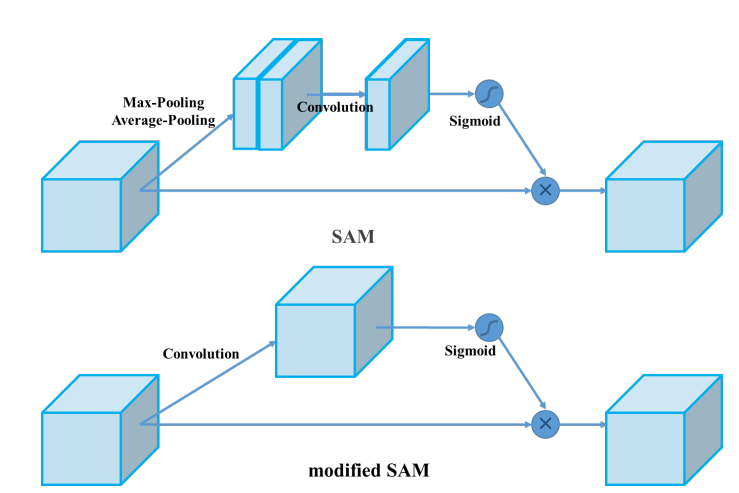
\includegraphics[width=1\textwidth]{img/modifedsam.png}
        \caption{Módulo de Atención Espacial Modificado \cite{yolov4}}
        \label{fig:sam}
    \end{figure}

\subsubsection{YOLOv5}

Poco después del lanzamiento de YOLOv4, se presentó YOLOv5 \cite{yolov5}, aunque sin documentación oficial al día de la redacción de este informe. Sin embargo, se conoce, por medio de foros y repositorios que lo han implementado, que cuenta los las siguientes mejoras:
\paragraph{Mejoras}
     \begin{enumerate}
		\item Es una implementación de YOLOv4 utilizando un framework en Python llamado Pytorch.
		\item Posee muchas optimizaciones algorítmicas y aritméticas.
        \item Se reduce sustancialmente el costo computacional de entrenamiento.
     \end{enumerate}

\paragraph{Memoria y FLOPS}
Cuando se habla de un modelo que es “liviano” se habla de su uso de la \textit{memoria RAM} necesaria para entrenarlo.
La cantidad necesaria viene dada por la cantidad de parámetros que el modelo seleccionado tiene para optimizar.
Si se mantiene constante la arquitectura, a mayor cantidad de parámetros, se suelen obtener mejores predicciones.
Si aumenta la cantidad de parámetros a optimizar, entonces también aumentan la cantidad de operaciones necesarias por iteración, lo que se traduce en mayor uso de CPU+GPU y por ende en tiempo de entrenamiento.
La unidad de medida para estas operaciones se conoce como \textit{FLOPs} (operaciones de punto flotante).\\
\hfill \break

\textbf{Comparación: Memoria y FLOPS} \\

En la siguiente tabla se ve claramente cómo el cambio de arquitectura en YOLO v5l (large), con una cantidad de parámetros incluso menor que YOLOv3, arroja resultados más performantes (mayor FPS) y precisos (mayor AP -precisión promedio-) que éste último.

\begin{figure}[h!]
    \centering
    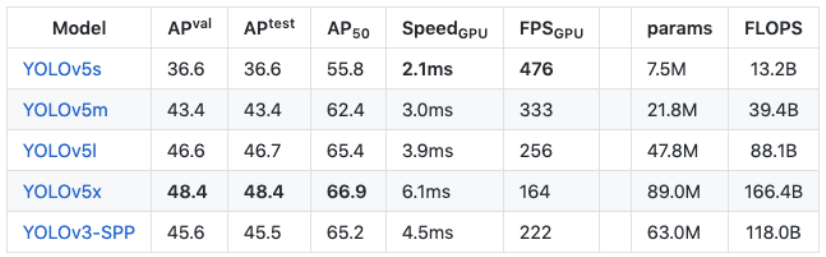
\includegraphics[width=1\textwidth]{img/tablaFLOPS.png}
    \caption{Arquitecturas: Memoria y FLOPS}
    \label{fig:tabla flops}
\end{figure}

\paragraph{Comparación de modelos de YOLOv5}
En la siguiente Figura (\ref{fig:yolo-v5-comparacion}), se puede observar como YOLOv5 hace un excelente rendimiento en la detección de objetos, especialmente el YOLOv5S, con más velocidad.
El objetivo es producir un modelo de detector de objetos que sea muy eficaz (eje Y) en relación con su tiempo de inferencia (eje X). Los resultados preliminares muestran que YOLOv5 lo hace muy bien con éste fin, en comparación con otras técnicas de vanguardia.

\begin{figure}[h!]
    \centering
    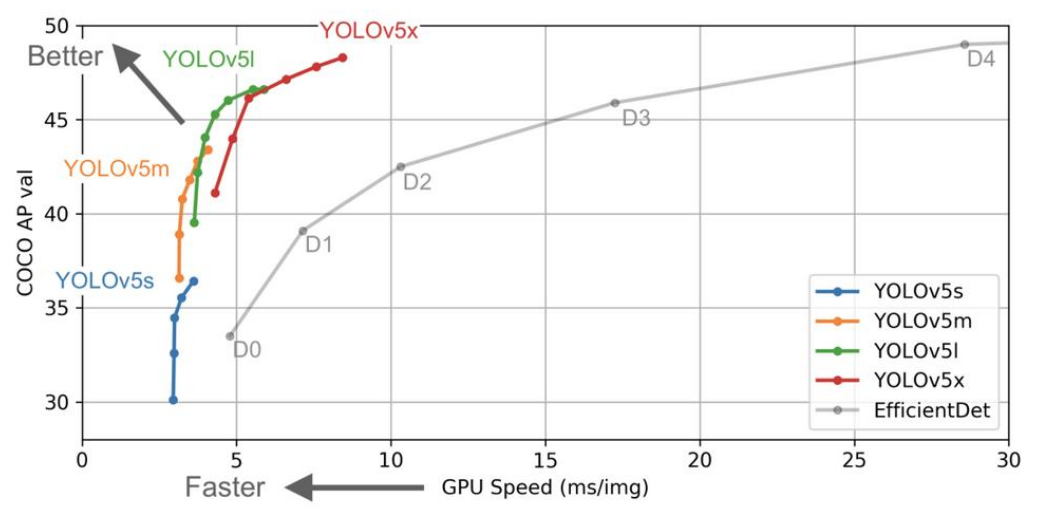
\includegraphics[width=1\textwidth]{img/Yolov5.png}
    \caption{YOLOv5 - Rendimiento}
    \label{fig:yolo-v5-comparacion}
\end{figure}

En resumen, YOLOv5 obtiene la mayor parte de su mejora de rendimiento de los procedimientos de entrenamiento de PyTorch, mientras que la arquitectura del modelo permanece muy cercana a YOLOv4.

\newpage

\chapter{Análisis del Diseño del Sistema}
\label{Análisis del Diseño del Sistema}

\section{Introducción}
Luego de haber adquirido una cantidad de conocimiento sobre Detección de Objetos en general y sobre el algoritmo de YOLO en particular, el presente capitulo 
investiga los problemas que tiene el área agropecuaria y la necesidad de detección y de localización de las silobolsas y mecanismos de riego por pivotes. Para esto, se realizó una entrevista con las partes interesadas o stakeholders en hacer uso de la aplicación resultante de este trabajo final, donde manifestaron su importancia. Luego se procede a analizar si las soluciones propuestas a las cuales se llegaron en la entrevista representan un caso de uso de Detección de Objetos. Por último, se especifican Componentes, Requerimientos y Comportamiento del sistema a implementar.
\begin{figure}[h!]
    \centering
    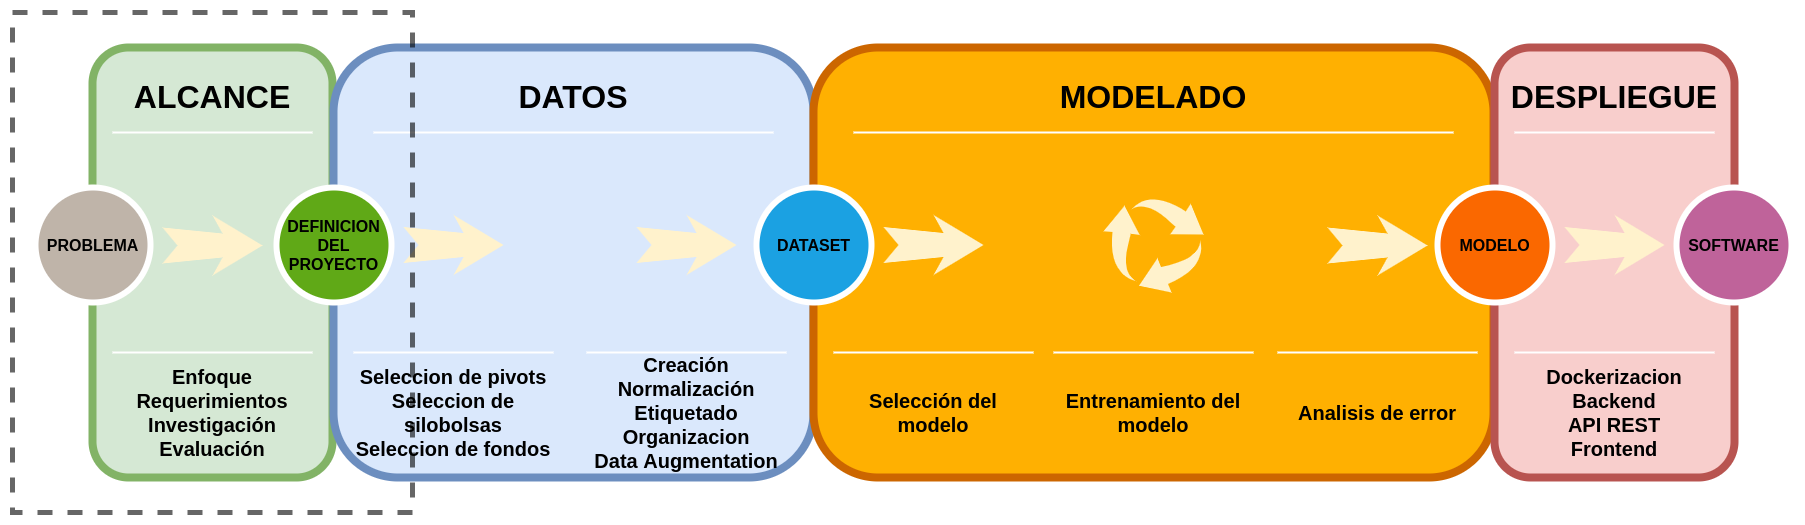
\includegraphics[width=1.2\textwidth,center]{img/Wokflow - alcance.drawio.png}
    \caption{Workflow: Alcance}
    \label{fig:workflow - alcance}
\end{figure}

\subsection{Entrevistas}


Las partes interesadas, como conocedores del área de las imágenes satelitales y del sector agropecuario, fueron entrevistadas con el objetivo de:
\begin{itemize}
    \item Entender las primeras especificaciones para el prototipo planteado en la sección \ref{Implementación}.
    \item Comprender mejor los problemas del sistema de riego que se usa en el campo, como así también el almacenamiento de los cereales, legumbres, entre otros.
    \item Hacer uso de éste prototipo y sus beneficios como parte de la solución de éstos problemas en un futuro.
\end{itemize}

De la charla, se plantearon los siguientes problemas:
\begin{itemize}
    \item Deforestaciones ilegales.
    \item Asentamientos ilegales y expropiaciones.
    \item Evasión impositivas en el rubro agropecuario.
    \item Abuso de los recursos hídricos.
\end{itemize}

La solución propuesta que surgió de la entrevista fue:
\begin{itemize}
    \item Debido a la fuerte influencia de algoritmos de Machine Learning de detección de objetos, se propuso hacer uso de ésta tecnología para desarrollar una aplicación que provea lo siguiente:
    \begin{itemize}
        \item Detectar múltiples objetos, es este caso, las silobolsas y los pivotes de riego.
        \item Dar la posición X e Y del objeto en la imagen (o su centro) y dibujar un rectángulo a su alrededor.
        \item La posibilidad de detectar “a tiempo”.  Ésta es una característica que se debe tener en cuenta si por ejemplo se quiere hacer detección en tiempo real sobre vídeo. Ésto es posible gracias a la velocidad y precisión para la inferencia que los detectores de objetos proveen.
    \end{itemize}
\end{itemize}

\subsection{Motivación e Importancia del proyecto}

Ante las preocupaciones anteriormente planteadas, se propone una solución para satisfacer esas necesidades que no estaban cubiertas, por lo cual se enumeran a continuación las motivaciones que se presentaron para llevarlo a cabo:

\begin{enumerate}
    \item Elevar la inteligencia de la toma de acciones automáticas, por ejemplo, en un sistema de Dirección General de Rentas.
    \item Incorporar tecnologías novedosas y altamente populares en la industria al ámbito Agropecuario público.
    \item Ayudar a combatir irregularidades o deforestaciones detectándolas en tiempo real.
\end{enumerate}

\subsection{Casos de uso de Machine Learning - Detección de objetos}


Desde el éxito de Machine Learning y el nacimiento de numerosas aplicaciones que la usan, como el reconocimiento facial en tiempo real (celulares), sugerencias de compras, autos autónomos, entre otras, están, hoy en día, todas al alcance de cualquiera. Es una tecnología que está madura y es adoptada en la vida cotidiana.

Un claro ejemplo del alcance de la Inteligencia Artificial, es el motor de Google con aplicaciones de sistemas de inteligencia artificial y aprendizaje profundo, el cual ofrece respuestas adecuadas, tales como son las traducciones automáticas, las recomendaciones de vídeos, el reconocimiento de imágenes y su posterior geo-localización, y hasta la detección de SPAM (correo electrónico masivo no solicitado) en el correo electrónico.

Otro impacto de esta tecnología, es en el futuro de la conducción con Piloto automático en coches Tesla \cite{tesla}, por ejemplo, que vienen de serie con una combinación de hardware y software avanzado capaz de ofrecer las funciones de Piloto automático y capacidades de conducción autónoma total basado en una IA (Inteligencia Artificial) para la visión y la planificación.


\subsection{Funcionalidades}

Luego de la entrevista y de la evaluación del caso de uso, se consideran necesarias las siguientes funcionalidades para el prototipo:
\begin{itemize}
    \item El prototipo debe consistir de una API con una interfaz amigable para que cualquier usuario pueda procesar una imagen.
    \item El prototipo debe ser capaz que recibir imágenes de diferentes tamaños y características, ya sea por unidad o por cantidad en archivos comprimidos. A las que se le va aplicar el algoritmo de detección.
    \item El prototipo debe proporcionar como resultado del procesamiento, una imagen con con los objetos detectados remarcados con cuadros delimitadores y su localización en coordenadas (x,y). 
\end{itemize}

Este prototipo se realiza con una una API de REST, o API de RESTful \cite{api}, la cual es una interfaz de programación de aplicaciones (API o API web), que se ajusta a los límites de la arquitectura REST y permite la interacción con los servicios web de RESTful.

En otras palabras, las APIs le permiten interactuar con una computadora o un sistema para obtener datos o ejecutar una función, de manera que el sistema comprenda la solicitud y la cumpla. Suele considerarse como el contrato entre el proveedor de información y el usuario, donde se establece el contenido que se necesita por parte del consumidor (la llamada) y el que requiere el productor (la respuesta). \\

\subsection{Definición de los Componentes}

Con el fin de implementar las funcionalidades descritas en la sección anterior, en primer lugar se definen los componentes del prototipo en su totalidad.

\begin{enumerate}

    \item \textbf{Modelo de Machine Learning}: Se necesita de un Modelo de Machine Learning que sea re-entrenable para detectar las clases de pivotes y de silobolsas. Que tenga un gran rendimiento en la detección de objetos para así cumplir con las exigencias en los cortos tiempos de inferencia deseados. Además, que sea liviano, para poder ser desplegado en un amplia variedad de sistemas, desde embebidos hasta clústeres.

    \item \textbf{Desarrollo de una API}: Se requiere de un proceso de continuo funcionamiento que sea capaz de recibir consultas, procesar los datos recibidos, disparar la ejecución del modelo para la inferencia y enviar mensajes al usuario final, ya sea con los resultados de detección de su consulta o bien notificar sobre la ocurrencia de algún error. En éste sentido, optar por el desarrollo de un API REST fue lo más óptimo, debido a su facilidad en la implementación y la amplia documentación disponible, sea cual sea el framework y/o lenguaje seleccionado para su desarrollo.

    \item \textbf{Desarrollo de una GUI}: Se precisa de una interfaz gráfica, que sea amigable para cualquier usuario y que sea capaz de generar consultas con los requerimientos del usuario y comunicarlas con el backend para su posterior procesamiento. A su vez, debe ser capaz de transmitir la información recibida por el backend de manera clara al usuario. Es por eso, que se optó por desarrollar un Frontend, representado por una página web, una vez más, beneficiándose en la rapidez en su implementación y el acceso a documentación detallada, sea cual sea el framework y/o lenguaje seleccionado para su desarrollo.

    \item \textbf{Diagrama general de la arquitectura}
    \begin{figure}[h!]
        \centering
        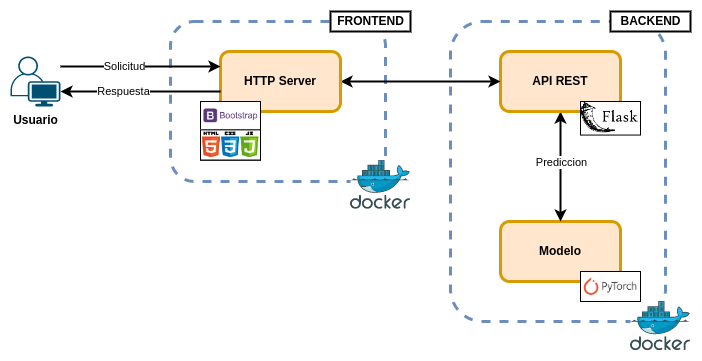
\includegraphics[width=1\textwidth,center]{img/BE - API - FE.drawio.png}
        \caption{Arquitectura del Software Implementado}
        \label{fig:be - api - fe}
    \end{figure}
\end{enumerate}

\subsubsection{Selección de los Componentes}
\begin{enumerate}

    \item \textbf{Elección del Modelo de Machine Learning:} 
    Luego del análisis y comparaciones entre los rendimientos de los diferentes modelos de ML más usados, se optó por una primera elección de YOLOv3 \cite{yolov3}. Se realizaron pruebas con diferentes sub-versiones del mismo (ej.: tiny, medium, large), donde variaba la profundidad de su arquitectura de red neuronal, afectando la precisión y los tiempos en las inferencias. Para éste modelo, se tomó mucho tiempo para re-entrenarlo y tratar de mejorar su precisión: aplicando diferentes técnicas de data augmentation sobre el dataset; modificando los hiper-parámetros del modelo; y hasta modificando secciones de su arquitectura de red neuronal, pero sin obtener los resultados esperados. Se tenían problemas para detectar objetos muy pequeños (silobolsas) junto a los objetos grandes (pivotes), o con diferentes texturas y colores, por lo que se optó por continuar con una versión más reciente del mismo: YOLOv5 \cite{yolov5}, que contaba con mejoras respecto a la versión 3, gracias a que se trata de un proyecto muy activo y en continuo desarrollo. Finalmente, éste fue el modelo elegido luego de realizar varias pruebas y mejoras con cambios en la configuración, modificando hiper parámetros con el con el fin de obtener mejores resultados, otorgando un excelente rendimiento y precisión en la detección de objetos, en comparación a sus alternativas (otras versiones de YOLO u otros modelos de ML).
    
    \item \textbf{Elección del lenguaje de programación:} El framework empleado para el entrenamiento y en el cual está basado el proyecto oficial de YOLOv5 \cite{yolov5}, es Python + Pytorch. En la selección del lenguaje con el cual se desarrollarían los scripts de diversa índole que fueran surgiendo en el desarrollo del proyecto, los lenguajes de programación conocidos, tales como C/C++ o JAVA, fueron descartados, ante la opción de Python, dada la mayor familiaridad y experiencia con dicho lenguaje, y a la amplia variedad de librerías orientadas al tratamiento de imágenes y datos que éste ofrece.
    
    \item \textbf{Elección para el desarrollo de una API:} Para el desarrollo del Backend, se optó por modificar y ampliar las funcionalidades que el repositorio oficial de YOLOv5 brindaba. El mismo, esta basado en Python+Flask, y la familiaridad y el conocimiento previo con dichos lenguaje y framework, la hacían una gran opción sobra la cual seguir desarrollando. Originalmente, ofrecía una implementación muy limitada para la clase de uso que se pretendía dar, y es por estos motivos, que se decidió trabajar sobre ésta base y agregarle las funcionalidades necesarias para cumplir con los objetivos del proyecto.
    En cuanto al servidor web necesario para desplegar y exponer un servicio continuo de comunicación, se optó por desarrollar el software en JavaScript. Ésta elección fue fundada en el hecho tener experiencia previa trabajando con dicho lenguaje, y las bondades que éste ofrece, para el desarrollo de éste tipo de aplicaciones web, frente a sus alternativas (Python o JAVA). JavaScript es, entonces, el código cliente que invoca al servidor, pero para que sea accesible a través de Internet es necesario continuar con el desarrollo de una API REST que permita llamar las funciones con métodos HTML. La herramienta elegida para proseguir con esa tarea es Node.js, que es un entorno en tiempo de ejecución multiplataforma para la capa del servidor basado en JavaScript, sobre el cual se tiene experiencia previa y se dispone de mucha documentación detallada online. Node.js es, a su vez, un entorno controlado por eventos, diseñado para crear aplicaciones escalables, permitiendo establecer y gestionar múltiples conexiones al mismo tiempo y flexibilidad para aplicaciones web y APIs, convirtiéndolo en el candidato más óptimo para el desarrollo de esta funcionalidad de la API.
    
    \item \textbf{Elección para el desarrollo de una GUI:} La API, públicamente expuesta a Internet, necesita un Frontend, o una interfaz web, que permita acceder a ella. Su funcionalidad consiste en obtener información de la API y mostrarla de forma entendible para el usuario, como también, obtener datos ingresados por el mismo y enviarlos para su procesamiento a la API.
    Para lograr eso, frente a la falta de experiencia específica previa en el desarrollo de GUIs, a excepción de HTML básico, se decidió utilizar Bootstrap \cite{bootstrap}, por su facilidad de uso y amplia disponibilidad de documentación y guías online. Usando ésta herramienta, las páginas adaptan su contenido de forma dinámica a medida que reciben entradas del usuario, en vez de descargar páginas nuevas de un servidor. Además, proporciona plantillas para CSS y HTML, que facilitan la colocación y el diseño de la página, las fuentes, los botones y los elementos de navegación, de modo que implementar con ella un diseño web moderno resulta sencillo.  
    
\end{enumerate}

\newpage
\subsection{Definición de los Requerimientos}

Para especificar el funcionamiento general del sistema, se va a hacer uso del lenguaje de modelado UML. Si bien se trata del desarrollo de un sistema distribuido con una variedad de protocolos y tecnologías, el prototipo final es un producto de software, por lo cual un modelado en SysML \cite{sysml} no se consideró.

Antes de plantear los requerimientos, primero es necesario definir un diagrama de casos de uso, como se ve en la Figura \ref{fig:diagrama-casos-de-uso}. En el diagrama se puede observar que el objetivo principal es brindarle al usuario un sistema de detección de objetos sobre imágenes satelitales.


\subsubsection {Diagrama de casos de uso}

\begin{figure}[h!]
    \centering
    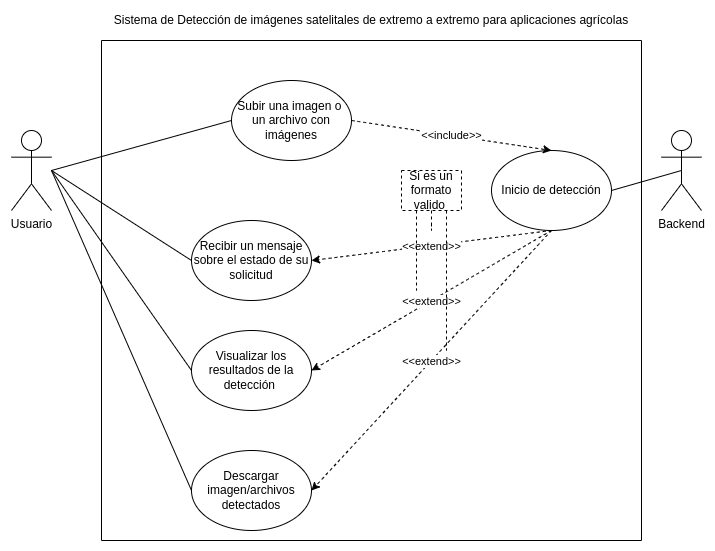
\includegraphics[width=1\textwidth]{img/Diagrama de Casos de usos.drawio (1).png}
    \caption{Diagrama de Caso de usos}
    \label{fig:diagrama-casos-de-uso}
\end{figure}

Con el diagrama de caso de uso elaborado se pueden definir los siguientes requerimientos de usuario, definidos en el Cuadro \ref{requser}:

\begin{table}[h!]
    \begin{tabular}{ | p{1cm} |p{11cm}| }
        \hline
        \rowcolor[HTML]{d6d8ff}
        R-01 & Cargar una imagen nueva al sistema.\\
        \hline
        R-02 & Verificar la presencia de una imagen cargada.\\
        \hline
        \rowcolor[HTML]{d6d8ff}
        R-03 & En caso de que sea un formato erróneo, mostrar un mensaje del error y debe ser posible volver a cargar una nueva imagen.\\
        \hline
        R-04 & Visualizar todas las imágenes cargadas y posteriormente un historial de las analizadas.\\
        \hline
        \rowcolor[HTML]{d6d8ff}
        R-05 & Analizar la imagen cargada, obtener información de la misma y el sistema debe informar si se encontró algún objeto o no.\\
        \hline
        R-06 & Descargar la imagen ya analizada.\\
        \hline
    \end{tabular}
    \caption{Requerimientos de Usuario}
    \label{requser}
\end{table}

\newpage
Luego es posible definir los requerimientos funcionales para cada uno de los componentes descritos anteriormente: la API y la interfaz gráfica. Los cuales se encuentran en los Cuadros \ref{reqapi} y \ref{reqfend} respectivamente. Los Requerimientos No funcionales se definieron en el Cuadro \ref{reqnf}.

\begin{table}[h!]
    \begin{tabular}{ | p{2cm} |p{10cm}| }
        \hline
        \rowcolor[HTML]{d6d8ff}
        RF-API-01 & Disponer de un endpoint para acceder a los servicios de detección.\\
        \hline
        RF-API-02 & Soportar una imagen y/o un archivo comprimido con imágenes.\\
        \hline
        \rowcolor[HTML]{d6d8ff}
         RF-API-03 & Realizar la detección de silobolsas y pivotes de riego sobre los archivos recibidos.\\
        \hline
         RF-API-04 & Retornar un archivos con la/s imágen/es con los objetos detectados.\\
        \hline
        \rowcolor[HTML]{d6d8ff}
         RF-API-05 & Retornar información adicional sobre la detección y el sistema donde fue ejecutado.\\
        \hline
    \end{tabular}\\
    \caption{Requerimientos Funcionales de la API}
    \label{reqapi}
\end{table}

\begin{table}[h!]
    \begin{tabular}{ | p{2cm} |p{10cm}| }
        \hline
        \rowcolor[HTML]{d6d8ff}
        RF-FE-01 & Mostrar información sobre el sistema y sus desarrolladores.\\
        \hline
        RF-FE-02 & Admitir carga de archivos.\\
        \hline
        \rowcolor[HTML]{d6d8ff}
        RF-FE-03 & Mostrar la imagen con los objetos detectados.\\
        \hline
        RF-FE-04 & Mostrar información de la detección.\\
        \hline
        \rowcolor[HTML]{d6d8ff}
        RF-FE-05 & Visualizar historial de la detecciones anteriores.\\
        \hline
        RF-FE-06 & Permitir la descarga de archivos.\\
        \hline
    \end{tabular}\\
    \caption{Requerimientos Funcionales del Frontend}
    \label{reqfend}
\end{table}

\begin{table}[h!]
    \begin{tabular}{ | p{2cm} |p{10cm}| }
        \hline
        \rowcolor[HTML]{d6d8ff}
        RNF-01 & Tiempo de detección menor a 100ms por imagen.\\
        \hline
        RNF-02 & Presentar una interfaz amigable para cualquier usuario.\\
        \hline
        \rowcolor[HTML]{d6d8ff}
        RNF-03 & Soportar diferentes formatos de archivos. \\
        \hline
        RNF-04 & Capacidad de ser desplegado fácilmente en diferentes sistemas\\
        \hline
        \rowcolor[HTML]{d6d8ff}
        RNF-05 & La API debe desarrollarse en Node.js y para la interfaz gráfica se debe usar CSS, HTML y JavaScript.\\
        \hline
    \end{tabular}\\
    \caption{Requerimientos No Funcionales del Sistema}
    \label{reqnf}
\end{table}

\newpage
Para comprender mejor cual es la relación estructural entre las diferentes tecnologı́as empleadas en el prototipo, se ofrece un diagrama de componentes, realizado en la Figura \ref{fig:componentes}. Se distinguen 3 componentes principales:
\begin{itemize}
    \item El Frontend donde se encuentra nuestra página web.
    \item La aplicación - API REST.
    \item El Modelo de Machine Learning - YOLOv5, donde los últimos dos componentes conforman el Backend.
\end{itemize}

\begin{figure}[h!]
    \centering
    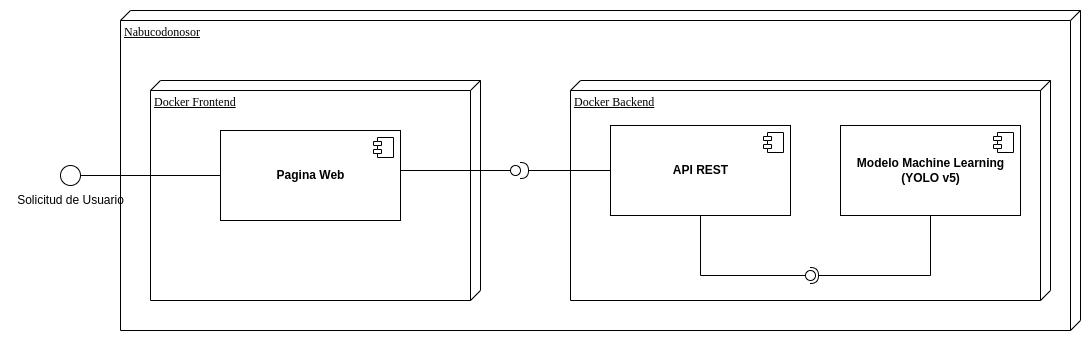
\includegraphics[width=1\textwidth]{img/Diagrama de Componentes.drawio.png}
    \caption{Diagrama de Componentes}
    \label{fig:componentes}
\end{figure}

\newpage
\subsection{Definición del Comportamiento}

Para entender cómo interactúan los componentes diagramados, se emplea un diagrama de secuencia en la Figura \ref{fig:secuencia}, en el cual se muestra el flujo de mensajes para el caso de subir una imagen a analizar y su posterior descarga, como también para verificar la validez del formato de una imagen y en caso de ser válido, proveer los resultados de las detecciones correspondientes.

\begin{figure}[h!]
    \centering
    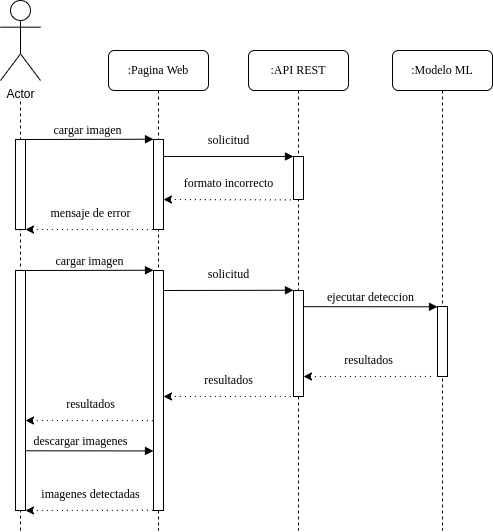
\includegraphics[width=1\textwidth]{img/Diagrama de Secuencia.drawio.png}
    \caption{Diagrama de Secuencia}
    \label{fig:secuencia}
\end{figure}


\subsection{Riesgos}

La evaluación de riesgos de un proyecto busca detectar posibles eventos no deseados que puedan perjudicar o amenazar al proyecto, con el objetivo de minimizarlos o controlar su impacto sobre el proyecto.

En la presente sección se establecen diferentes criterios para identificar posibles riesgos, asignar prioridades a los mismos, evaluar su probabilidad y encontrar estrategias que permitan resolver los mismos o minimizar sus efectos.


\subsubsection{Criterios}

Los riesgos se clasifican según dos criterios: su probabilidad y la gravedad en el caso de su ocurrencia. A continuación, figuran las probabilidades y gravedades que se tuvieron en cuenta según Ian Sommerville en su libro Software Engineering \cite{sommerville}:

\begin{enumerate}
    \item Riesgo muy bajo (menor a 10 \%)
    \item Riesgo bajo (10 - 25 \%)
    \item Riesgo moderado (25 - 50 \%)
    \item Riesgo alto (50 - 75 \%)
    \item Riesgo muy alto (mayor a 75 \%)
\end{enumerate}

\begin{enumerate}
    \item Efectos insignificantes
    \item Efectos tolerables
    \item Efectos graves
    \item Efectos catastróficos
\end{enumerate}

La combinación de ambos criterios permite detectar y priorizar los riesgos teniendo en cuenta ambos factores, y se consideran a los riesgos dentro del área verde como los de menor prioridad, los riesgos en el área amarilla como de prioridad intermedia y los riesgos en el área roja como de prioridad alta, como se muestra en el Cuadro \ref{probriesgos}.

\begin{table}[h]
    \begin{tabular}{ | m{3cm} | m{3cm}| m{2cm} | m{2cm} |m{2cm} |}
        \hline
        Probabilidad-Efecto & Insignificante & Tolerable &Grave & Catastrófico\\
        \hline
        Muy baja& \cellcolor[HTML]{84D65C} & \cellcolor[HTML]{84D65C}&\cellcolor[HTML]{84D65C} &\cellcolor[HTML]{FFFF00}\\
        \hline
        Baja & \cellcolor[HTML]{84D65C} & \cellcolor[HTML]{84D65C}&\cellcolor[HTML]{FFFF00} &\cellcolor[HTML]{FFFF00}\\
        \hline
        Moderada& \cellcolor[HTML]{84D65C} &\cellcolor[HTML]{FFFF00} &\cellcolor[HTML]{FFFF00} &\cellcolor[HTML]{FF3333} \\
        \hline
        Alta  &\cellcolor[HTML]{FFFF00}  &\cellcolor[HTML]{FFFF00} & \cellcolor[HTML]{FF3333} &\cellcolor[HTML]{FF3333} \\
        \hline
        Muy alta & \cellcolor[HTML]{FFFF00} &\cellcolor[HTML]{FF3333}  & \cellcolor[HTML]{FF3333} &\cellcolor[HTML]{FF3333} \\
        \hline
    \end{tabular}\\
    \caption{Probabilidad de Riesgos Vs Efecto}
    \label{probriesgos}
\end{table}

\subsubsection{Identificación de Riesgos}

En la etapa de la gestión de riesgos, se buscan los posibles riesgos relacionados al proyecto escritos en el Cuadro \ref{riesgosproyecto}, distinguiendo las siguientes categorías :
\begin{itemize}
    \item \textbf{Riesgos de tecnologı́a}: Riesgos relacionados la hardware o software con el que se está desarrollando el presente proyecto.
    \item \textbf{Riesgos personales:} Relacionados con lo personal del equipo de desarrollo.
    \item \textbf{Riesgos de requerimientos:} Surgen de modificaciones de los requerimientos.
    \item \textbf{Riesgos de estimación:} relacionados a la estimación de recursos requeridos o estimación de tiempo para el desarrollo del proyecto.
\end{itemize}

\begin{table}[h]
    \begin{tabular}{ | m{1.5cm} | m{7cm}| m{3.5cm}  |}
        \hline
        \rowcolor{lightgray}
        Código & Descripción & Tipo de Riesgo \\
        \hline
        Riesgo-01 & Problemas de funcionamiento o fuera de servicio de la Máquina donde se desarrolla el proyecto  & Tecnológico \\
        \hline
        Riesgo-02 & Incompatibilidad de versiones o librerı́as instaladas en la máquina de desarrollo con los frameworks usados.  &Tecnológico \\
        \hline
        Riesgo-03 & Demoras durante el desarrollo del proyecto debido a trabajo u otros inconvenientes personales.  &  Personales y Estimación\\
        \hline
        Riesgo-04 & Errores en la implementación de los frameworks elegidos.  & Tecnológico, Requerimientos y Estimación\\
        \hline
        Riesgo-05 & Falta de conocimiento o documentación para el uso de los frameworks, del software o los lenguajes de programación elegidos.  & Estimación\\
        \hline
        Riesgo-06 & Rechazo de la implementación por parte del usuario final.  & Estimación\\
        \hline
    \end{tabular}\\
    \caption{Riesgos identificados para el proyecto}
    \label{riesgosproyecto}
\end{table}

\newpage
\subsubsection{Análisis de Riesgos}

En el Cuadro \ref{riesgosprobyefecto} se ordenaron los riesgos según su importancia, probabilidad y efecto.

\begin{table}[h!]
    \begin{tabular}{ | m{1.5cm} | m{4cm}|m{2cm}  | m{2cm}  | m{2cm}  |}
        \hline
        \rowcolor{lightgray}
        Código & Riesgo & Probabilidad & Efecto & Importancia \\
        \hline
        Riesgo-02 & Incompatibilidad de versiones o librerı́as instaladas en la máquina de desarrollo con los frameworks usados. & Moderada &Insignificante&
        \cellcolor[HTML]{84D65C} Prioridad baja \\
        \hline
        Riesgo-01 & Problemas de funcionamiento o fuera de servicio de la Máquina donde se desarrolla el proyecto & Baja &Grave & \cellcolor[HTML]{FFFF00} Prioridad Intermedia\\
        \hline
        Riesgo-05 & Falta de conocimiento o documentación para el uso de los frameworks, del software o los lenguajes de programación elegidos.
         & Alta   & Tolerable& \cellcolor[HTML]{FFFF00} Prioridad Intermedia\\
        \hline
        Riesgo-04  & Errores en la implementación de los frameworks elegidos.  & Alta  &Tolerable &\cellcolor[HTML]{FFFF00} Prioridad intermedia\\
        \hline
         Riesgo-03 & Demoras durante el desarrollo del proyecto debido a trabajo u otros inconvenientes personales.  & Alta  &Grave & \cellcolor[HTML]{FF3333} Prioridad alta\\
        \hline
        Riesgo-06 & Rechazo de la implementación por parte del usuario final.  & Alta  &Grave & \cellcolor[HTML]{FF3333} Prioridad alta\\
        \hline
    \end{tabular}\\
    \caption{Riesgos según su probabilidad y efecto}
    \label{riesgosprobyefecto}
\end{table}

\newpage
\subsubsection{Planificación de Riesgos}

En la presente sección se describen las estrategias para manejar cada riesgo identificado anteriormente, y se detallan en los Cuadros \ref{manejoriesgos1} y \ref{manejoriesgos2}.

\begin{table}[h!]
    \begin{tabular}{ | m{1.5cm} | m{5cm}| m{5cm} |}
        \hline
        \textbf{Código} & \textbf{Riesgo} & \textbf{Estrategias de Manejo del riesgo} \\
        \hline
        Riesgo-01 & Problemas de funcionamiento o fuera de servicio de la Máquina donde se desarrolla el proyecto  & \begin{itemize}
         \item Implementación de un respaldo de información en la nube con repositorios de Github.
            \item Realización de la operación \textit{git push} al repositorio diariamente o ante algún cambio. 
             \end{itemize}\\
        \hline
         Riesgo-02 & Incompatibilidad de versiones o librerı́as instaladas en la máquina de desarrollo con los frameworks usados.&  \begin{itemize}
         \item Lectura cuidadosa de tutoriales de instalación y pre-requisitos.     
         \item Uso de Docker para ganar mayor flexibilidad con versiones de librerı́as o lenguajes de programación. 
         \end{itemize} \\
        \hline
         Riesgo-03 & Demoras durante el desarrollo del proyecto debido a trabajo u otros inconvenientes personales.    
         & \begin{itemize} 
            \item Comunicación fluida con director y codirector del Proyecto.    
            \item Reducción de obligaciones laborales y extracurriculares. 
            \item Definición clara del alcance del proyecto para minimizar las posibles demoras de tiempo y trabajo.
          \end{itemize}\\
        \hline
        Riesgo-04 & Errores en la implementación de los frameworks elegidos.  &
        \begin{itemize} 
                    \item Implementación de métodos descritos en la documentación o páginas de seguimientos, como también foros oficiales.
                    \item Modificación o adaptación del requerimiento y su implementación.
                \end{itemize}\\
        \hline
    \end{tabular}\\
    \caption{Estrategias de manejo de riesgos - Parte 1}
    \label{manejoriesgos1}
\end{table}


\begin{table}[h!]
    \begin{tabular}{ | m{1.5cm} | m{5cm}| m{5cm} |}
        \hline
        \textbf{Código} & \textbf{Riesgo} & \textbf{Estrategias de Manejo del riesgo} \\
        \hline
         Riesgo-05 & Falta de conocimiento o documentación para el uso de los frameworks, del software o los lenguajes de programación elegidos.&  \begin{itemize} 
                    \item Lectura de tutoriales y realización de cursos cortos para lograr una introducción en temas cuyo desconocimiento impida el avance del proyecto.
                    \item Empleo y modificación/adaptación de ejemplos previstos para el aprendizaje.
                    \item Búsqueda de explicaciones adicionales en foros de usuarios como StackOverflow \cite{stackoverflow}.
                    \item Consultas a programadores o profesionales experimentados en los campos en cuestión.
                \end{itemize}\\
        \hline
        Riesgo-06 &Rechazo de la implementación por parte del usuario final.  & 
        \begin{itemize} 
            \item Explicación de la tecnologı́a empleada y proporcionar manual de usuario para su uso.
            \item  Prueba de piloto para identificar mejoras en cuanto a la usabilidad y posibilidad de mejoras en un futuro.
                \end{itemize}\\
        \hline
    \end{tabular}\\
    \caption{Estrategias de manejo de riesgos - Parte 2}
    \label{manejoriesgos2}
\end{table}

\newpage
\subsection{Control de Versiones }
Git es una herramienta para mejorar la colaboración entre varios programadores. Usar un repositorio permite tener acceso remoto al proyecto desde cualquier equipo, teniendo ası́ una copia de seguridad del proyecto completo en la nube. A su vez, se mantiene un historial de versiones y en caso de ser necesario, volver a una versión anterior o comparar las diferencias entre dos versiones distintas.

Para el control de versiones, se utilizó un repositorio de Github disponible bajo la URL:  \url{https://github.com/gianfrancob/detector_pivotes_silobolsas}
\newpage

\input{Chapters/Implementación}
\input{Chapters/Validación}
\input{Chapters/Conclusión}

%---------------------------------------------------------------
%	THESIS CONTENT - APPENDICES
%---------------------------------------------------------------
\addtocontents{toc}{\vspace{2em}} % Add a gap in the Contents, for aesthetics
\newpage
    \chapter{Apéndice}
    \label{Apéndice}
    \section{Imágenes Dataset} \label{anexo:dataset}

\begin{figure}
    \centering
    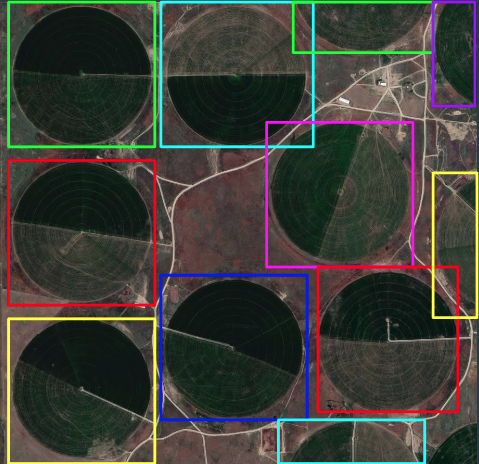
\includegraphics[width=0.9\textwidth]{img/pivot etiquetado manual - 1.png}
    \caption{Pívot etiquetado manualmente}
    \label{Pivot etiquetado manualmento 1}
\end{figure}

\begin{figure}
    \centering
    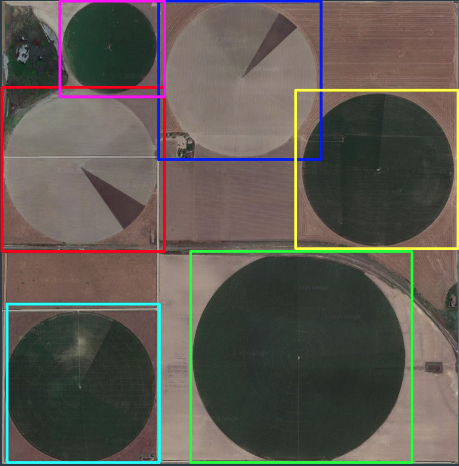
\includegraphics[width=0.9\textwidth]{img/pivot etiquetado manual - 2.png}
    \caption{Pívot etiquetado manualmente}
    \label{Pivot etiquetado manualmento 2}
\end{figure}

\begin{figure}
    \centering
    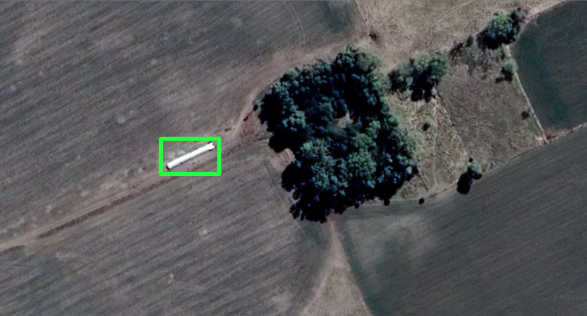
\includegraphics[width=0.9\textwidth]{img/silobolsa etiquetado manual - 1.png}
    \caption{Silobolsa etiquetado manualmente}
    \label{Silobolsa etiquetado manualmento 1}
\end{figure}

\begin{figure}
    \centering
    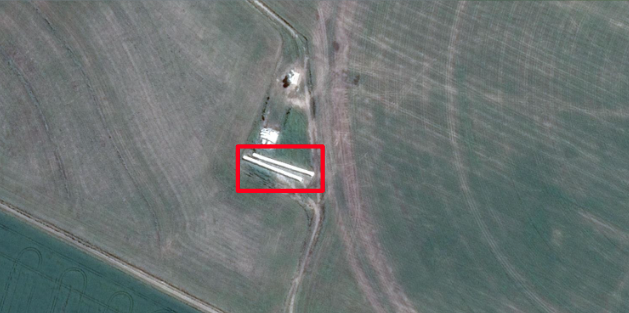
\includegraphics[width=0.9\textwidth]{img/silobolsa etiquetado manual - 2.png}
    \caption{Silobolsa etiquetado manualmente}
    \label{Silobolsa etiquetado manualmento 2}
\end{figure}

\begin{figure}
    \centering
    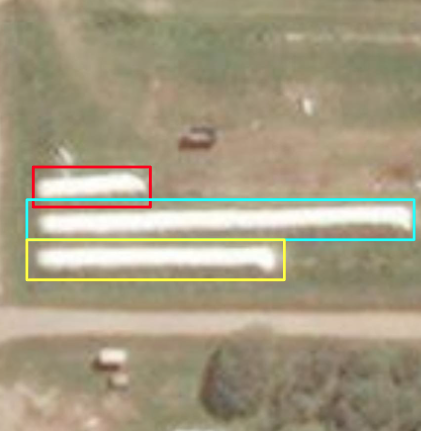
\includegraphics[width=0.9\textwidth]{img/silobolsa etiquetado manual - 3.png}
    \caption{Silobolsa etiquetado manualmente}
    \label{Silobolsa etiquetado manualmento 3}
\end{figure}

\begin{figure}
    \centering
    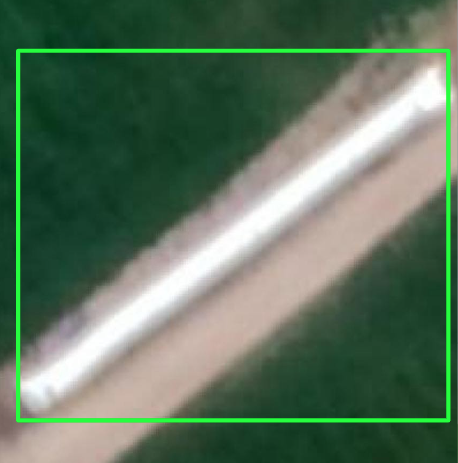
\includegraphics[width=0.9\textwidth]{img/silobolsa etiquetado manual - 4.png}
    \caption{Silobolsa etiquetado manualmente}
    \label{Silobolsa etiquetado manualmento 4}
\end{figure}

\begin{figure}
    \centering
    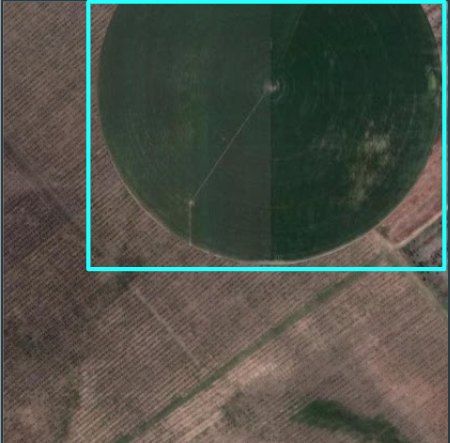
\includegraphics[width=0.9\textwidth]{img/pivot data aug - 1.png}
    \caption{Pívot generado con data augmentation}
    \label{Pivot generado con data augmentation 1}
\end{figure}

\begin{figure}
    \centering
    \includegraphics[width=0.9\textwidth]{img/pivot data aug - 2.png}
    \caption{Pívot generado con data augmentation}
    \label{Pivot generado con data augmentation 2}
\end{figure}

\begin{figure}
    \centering
    \includegraphics[width=0.9\textwidth]{img/pivot data aug - 3.png}
    \caption{Pívot generado con data augmentation}
    \label{Pivot generado con data augmentation 3}
\end{figure}

\begin{figure}
    \centering
    \includegraphics[width=0.9\textwidth]{img/silobolsa data aug - 1.png}
    \caption{Silobolsa generado con data augmentation}
    \label{Silobolsa generado con data augmentation 1}
\end{figure}

\begin{figure}
    \centering
    \includegraphics[width=0.9\textwidth]{img/silobolsa data aug - 2.png}
    \caption{Silobolsa generado con data augmentation}
    \label{Silobolsa generado con data augmentation 2}
\end{figure}

    \section{Manual de Usuario}
\subsection{Introducción}
En esta sección se detallan los pasos a seguir para el uso adecuado del software Detector de Pivotes de Riego y Silo bolsas en Imágenes Satelitales para aplicaciones agrícolas.

\subsection{Pre-requisitos}
Contar con Docker instalado en la computadora.

En el caso de no optar por el uso de Docker, se puede correr localmente de contar con los siguientes requerimientos:
\begin{itemize}
    \item Distribución Linux: Debian o Ubuntu preferentemente (o sus derivados).
    \item Python 3.7 o superior.
    \item Virtualenv.
\end{itemize}

\subsection{Instalación}
\begin{enumerate}
    \item Descargar o clonar el repositorio desde Github: \url{https://github.com/gianfrancob/detector_pivotes_silobolsas}
    \item Inicializar el contenedor Docker corriendo: 
    \begin{itemize}
            \item \textit{docker build -t detector\_pivotes\_silobolsas }
            \item \textit{docker run -p 5000:5000 --name test -it detector\_pivotes\_silobolsas}
    \end{itemize}
    
    \item En el caso de no optar por el uso de Docker, se puede correr localmente de la siguiente manera:
    \begin{itemize}
        \item Crear entorno virtual usando virtualenv: \textit{virtualenv venv}
        \item Activar el entorno: \textit{source ./venv/bin/activate}
        \item Instalar las dependencias en el entorno: \textit{pip install -r ./requirements.txt}
    \end{itemize}
    \item Iniciar el servicio backend: \textit{python ./utils/flask\_rest\_api/restapi\_pivot\_silobolsa.py --port 5000}
    \item Ingresar a la página abriendo en el navegador el siguiente fichero HTML: \textit{./utils/boostrap\_frontend/index.html}
\end{enumerate}

xt

\subsection{Ingresar a la página}
Para ejecución local, la dirección URL donde se encuentra la aplicación es: 
\textit{DIRECTORIO RAIZ/utils/boostrap\_frontend/index.html}

Para ejecución web, dependerá particularmente del tipo de despliegue implementado.

\subsection{Cargar una imagen}

\begin{figure}[b!]
    \centering
    \includegraphics[width=0.8\textwidth]{img/FE - upload file.png}
    \caption{Subir una imagen para analizar}
    \label{fig:subir imagen}
\end{figure}

Una vez en la página principal, dirigirse al botón "Seleccionar archivo" que se encuentra en la mitad de la misma y hacer clic en él para seleccionar una imagen o desde la computadora del usuario, los formatos soportados son .jpg, .png .

\subsubsection{Error en el formato de la imagen}

Si el formato de la imagen cargada esta dañado o es invalido, se mostrara el siguiente mensaje, como se muestra en la figura \ref{fig:error}:

\begin{figure}[h!]
    \centering
    \includegraphics[width=0.6\textwidth]{img/FE - upload error.png} 
    \caption{Error al subir una archivo de formato invalido}
    \label{fig:error}
\end{figure}

\subsection{Cargar varias imágenes} 

Para la opción del análisis de un conjunto de imágenes, previamente se debe crear un archivo de compresión con todas las imágenes en alguno de los siguientes formatos: RPM (.rpm), RAR (.rar), RZIP (.rz), TAR (.tar), XZ (.xz), ZIP (.zip, .jar), GZIP (.gz), 7z (.7z).

Luego, hacer clic en el botón "Seleccionar archivo" para subir el archivo con todas las imágenes a ser analizadas.

\textbf{Nota}: No debe salir ningún mensaje de error para continuar con el análisis,  ver imagen \ref{fig:error}

\subsection{Inicio de la detección} 

Una vez cargada la imagen o las imágenes en formatos validos, hacer clic en el botón \textbf{"Submit"}, para dar inicio a la detección. 

\begin{figure}[h!]
    \centering
    \includegraphics[width=0.6\textwidth]{img/FE - detection loading.png}
    \caption{Inicio de la detección - Loading}
    \label{fig:loading}
\end{figure}

El botón cambiara de nombre y aparece como "Loading", indicando que la detección esta en proceso. Como se puede apreciar en la Figura \ref{fig:loading}.


\subsection{Descarga de imágenes}

Una vez realizada la detección de los objetos, se va a mostrar como resultado las imágenes analizadas indicando la presencia de los objetos Silo bolsas o Riegos por Pívot junto con una tabla donde se detalla la información de la detección.

Luego, se habilitara un botón \textbf{"Download"} que al hacer clic en él, se procede a la descarga de la/s imágenes, como se ve en la Figura \ref{fig:bulk detection} y se debe seleccionar el archivo del destino como se muestra en la Figura \ref{fig:download file}

\begin{figure}[h!]
    \centering
    \includegraphics[width=0.93\textwidth]{img/FE - bulk detection.png}
    \caption{Detección de un archivo con imágenes comprimidas}
    \label{fig:bulk detection}
\end{figure}

\begin{figure}[h!]
\centering
    \includegraphics[width=1\textwidth]{img/FE - download file.png}
    \caption{Descarga de archivo con imágenes detectadas - Resultados}
    \label{fig:download file}
\end{figure}

\pagebreak

% Los manuales se elaboran en base a las necesidades de los usuarios de la empresa a la que se le ha realizado el sistema. Algunos pueden contener los siguientes apartados:

% Portada
% Índice
% Introducción
% Instalación del sistema
% Diagrama general del sistema
% Diagrama particular detallado
% Explicación genérica de las fases del sistema
% Iniciación al uso del sistema
% Manual de Referencia


% Las secciones de un manual de usuario2​ a menudo incluyen:

% Una página de portada.
% Una página de título y una página de derechos de autor.
% Un prefacio, que contiene detalles de los documentos relacionados y la información sobre cómo navegar por el manual del usuario.
% Una sección de propósito, que es más una descripción general que un resumen del objetivo del documento.
% Una sección de audiencia que indique explícitamente quién es la audiencia prevista a leer el manual, incluyendo la audiencia opcional.
% Una sección de alcance es crucial ya que también sirve como un descargo de responsabilidad, indicando lo que está fuera del alcance y lo que sí está cubierto.
% Una guía sobre cómo utilizar al menos las principales funciones del sistema, es decir, sus funciones básicas.
% Una sección de solución de problemas que detalla los posibles errores o problemas que pueden surgir, junto con la forma de solucionarlos.
% Una sección de preguntas frecuentes, donde encontrar más ayuda y datos de contacto.
% Un glosario y, para documentos más grandes, un índice.

% \end{appendices}

\backmatter

%---------------------------------------------------------------
%	THESIS CONTENT - BIBLIOGRAFIA
%---------------------------------------------------------------
\newpage
\bibliographystyle{splncs04}
\bibliography{bibfile}
\end{document}\grid